\documentclass[a4paper, 12pt]{article}

% packages
\usepackage{amssymb}
\usepackage[fleqn]{mathtools}
\usepackage{tikz}
\usepackage{enumerate}
\usepackage{bussproofs}
\usepackage{xcolor}
\usepackage[margin=1.3cm]{geometry}
\usepackage{logicproof}
\usepackage{diagbox}
\usepackage{listings}
\usepackage{graphicx}
\usepackage{lstautogobble}
\usepackage{hyperref}
\usepackage{multirow}
\usepackage{tipa}
\usepackage{pgfplots}
\usepackage{adjustbox}

% tikz libraries
\usetikzlibrary{
    decorations.pathreplacing,
    arrows,
    shapes,
    shapes.gates.logic.US,
    circuits.logic.US,
    calc,
    automata,
    positioning,
    intersections
}

\pgfplotsset{compat=1.16}

\pgfmathdeclarefunction{gauss}{2}{%
  \pgfmathparse{1/(#2*sqrt(2*pi))*exp(-((x-#1)^2)/(2*#2^2))}%
}

\allowdisplaybreaks % allow environments to break
\setlength\parindent{0pt} % no indent

% shorthand for verbatim
% this clashes with logicproof, so maybe fix this at some point?
\catcode`~=\active
\def~#1~{\texttt{#1}}

% code listing
\lstdefinestyle{main}{
    numberstyle=\tiny,
    breaklines=true,
    showspaces=false,
    showstringspaces=false,
    tabsize=2,
    numbers=left,
    basicstyle=\ttfamily,
    columns=fixed,
    fontadjust=true,
    basewidth=0.5em,
    autogobble,
    xleftmargin=3.0ex,
    mathescape=true
}
\newcommand{\dollar}{\mbox{\textdollar}} %
\lstset{style=main}

% augmented matrix
\makeatletter
\renewcommand*\env@matrix[1][*\c@MaxMatrixCols c]{%
\hskip -\arraycolsep
\let\@ifnextchar\new@ifnextchar
\array{#1}}
\makeatother

% ceiling / floor
\DeclarePairedDelimiter{\ceil}{\lceil}{\rceil}
\DeclarePairedDelimiter{\floor}{\lfloor}{\rfloor}

% custom commands
\newcommand{\indefint}[2]{\int #1 \, \mathrm{d}#2}
\newcommand{\defint}[4]{\int_{#1}^{#2} #3 \, \mathrm{d}#4}
\newcommand{\pdif}[2]{\frac{\partial #1}{\partial #2}}
\newcommand{\dif}[2]{\frac{\mathrm{d}#1}{\mathrm{d}#2}}
\newcommand{\limit}[2]{\raisebox{0.5ex}{\scalebox{0.8}{$\displaystyle{\lim_{#1 \to #2}}$}}}
\newcommand{\limitsup}[2]{\raisebox{0.5ex}{\scalebox{0.8}{$\displaystyle{\limsup_{#1 \to #2}}$}}}
\newcommand{\summation}[2]{\sum\limits_{#1}^{#2}}
\newcommand{\product}[2]{\prod\limits_{#1}^{#2}}
\newcommand{\intbracket}[3]{\left[#3\right]_{#1}^{#2}}
\newcommand{\laplace}{\mathcal{L}}
\newcommand{\fourier}{\mathcal{F}}
\newcommand{\mat}[1]{\boldsymbol{#1}}
\renewcommand{\vec}[1]{\boldsymbol{#1}}
\newcommand{\rowt}[1]{\begin{bmatrix}
    #1
\end{bmatrix}^\top}
\DeclareMathOperator*{\argmax}{argmax}
\DeclareMathOperator*{\argmin}{argmin}

\newcommand{\lto}[0]{\leadsto\ }

\newcommand{\ulsmash}[1]{\underline{\smash{#1}}}

\newcommand{\powerset}[0]{\wp}
\renewcommand{\emptyset}[0]{\varnothing}

\makeatletter
\newsavebox{\@brx}
\newcommand{\llangle}[1][]{\savebox{\@brx}{\(\m@th{#1\langle}\)}%
  \mathopen{\copy\@brx\kern-0.5\wd\@brx\usebox{\@brx}}}
\newcommand{\rrangle}[1][]{\savebox{\@brx}{\(\m@th{#1\rangle}\)}%
  \mathclose{\copy\@brx\kern-0.5\wd\@brx\usebox{\@brx}}}
\makeatother
\newcommand{\lla}{\llangle}
\newcommand{\rra}{\rrangle}
\newcommand{\la}{\langle}
\newcommand{\ra}{\rangle}
\newcommand{\crnr}[1]{\text{\textopencorner} #1 \text{\textcorner}}
\newcommand{\bnfsep}[0]{\ |\ }
\newcommand{\concsep}[0]{\ ||\ }

\newcommand{\axiom}[1]{\AxiomC{#1}}
\newcommand{\unary}[1]{\UnaryInfC{#1}}
\newcommand{\binary}[1]{\BinaryInfC{#1}}
\newcommand{\trinary}[1]{\TrinaryInfC{#1}}
\newcommand{\quaternary}[1]{\QuaternaryInfC{#1}}
\newcommand{\quinary}[1]{\QuinaryInfC{#1}}
\newcommand{\dproof}[0]{\DisplayProof}
\newcommand{\llabel}[1]{\LeftLabel{\scriptsize #1}}
\newcommand{\rlabel}[1]{\RightLabel{\scriptsize #1}}

\newcommand{\ttbs}{\char`\\}
\newcommand{\lrbt}[0]{\ \bullet\ }

% colours
\newcommand{\violet}[1]{\textcolor{violet}{#1}}
\newcommand{\blue}[1]{\textcolor{blue}{#1}}
\newcommand{\red}[1]{\textcolor{red}{#1}}
\newcommand{\teal}[1]{\textcolor{teal}{#1}}

% reasoning proofs
\usepackage{ltablex}
\usepackage{environ}
\keepXColumns
\NewEnviron{reasoning}{
    \begin{tabularx}{\textwidth}{rlX}
        \BODY
    \end{tabularx}
}
\newcommand{\proofline}[3]{$(#1)$ & $#2$ & \hfill #3 \smallskip \\}
\newcommand{\proofarbitrary}[1]{& take arbitrary $#1$ \smallskip \\}
\newcommand{\prooftext}[1]{\multicolumn{3}{l}{#1} \smallskip \\}
\newcommand{\proofmath}[3]{$#1$ & = $#2$ & \hfill #3 \smallskip \\}
\newcommand{\prooftherefore}[1]{& $\therefore #1$ \smallskip \\}
\newcommand{\proofbc}[0]{\prooftext{\textbf{Base Case}}}
\newcommand{\proofis}[0]{\prooftext{\textbf{Inductive Step}}}

% ER diagrams
\newcommand{\nattribute}[4]{
    \node[draw, state, inner sep=0cm, minimum size=0.2cm, label=#3:{#4}] (#1) at (#2) {};
}
\newcommand{\mattribute}[4]{
    \node[draw, state, accepting, inner sep=0cm, minimum size=0.2cm, label=#3:{#4}] (#1) at (#2) {};
}
\newcommand{\dattribute}[4]{
    \node[draw, state, dashed, inner sep=0cm, minimum size=0.2cm, label=#3:{#4}] (#1) at (#2) {};
}
\newcommand{\entity}[3]{
    \node[] (#1-c) at (#2) {#3};
    \node[inner sep=0cm] (#1-l) at ($(#1-c) + (-1, 0)$) {};
    \node[inner sep=0cm] (#1-r) at ($(#1-c) + (1, 0)$) {};
    \node[inner sep=0cm] (#1-u) at ($(#1-c) + (0, 0.5)$) {};
    \node[inner sep=0cm] (#1-d) at ($(#1-c) + (0, -0.5)$) {};
    \draw
    ($(#1-c) + (-1, 0.5)$) -- ($(#1-c) + (1, 0.5)$) -- ($(#1-c) + (1, -0.5)$) -- ($(#1-c) + (-1, -0.5)$) -- cycle;
}
\newcommand{\relationship}[3]{
    \node[] (#1-c) at (#2) {#3};
    \node[inner sep=0cm] (#1-l) at ($(#1-c) + (-1, 0)$) {};
    \node[inner sep=0cm] (#1-r) at ($(#1-c) + (1, 0)$) {};
    \node[inner sep=0cm] (#1-u) at ($(#1-c) + (0, 1)$) {};
    \node[inner sep=0cm] (#1-d) at ($(#1-c) + (0, -1)$) {};
    \draw
    ($(#1-c) + (-1, 0)$) -- ($(#1-c) + (0, 1)$) -- ($(#1-c) + (1, 0)$) -- ($(#1-c) + (0, -1)$) -- cycle;
}

% AVL Trees
\newcommand{\avltri}[4]{
    \draw ($(#1)$) -- ($(#1) + #4*(0.5, -1)$) -- ($(#1) + #4*(-0.5, -1)$) -- cycle;
    \node at ($(#1) + #4*(0, -1) + (0, 0.5)$) {#3};
    \node at ($(#1) + #4*(0, -1) + (0, -0.5)$) {#2};
}

% RB Trees
\tikzset{rbtr/.style={inner sep=2pt, circle, draw=black, fill=red}}
\tikzset{rbtb/.style={inner sep=2pt, circle, draw=black, fill=black}}

% Samples
\tikzset{spos/.style={inner sep=2pt, circle, draw=black, fill=blue!20}}
\tikzset{sneg/.style={inner sep=2pt, circle, draw=black, fill=red!20}}

% Joins
\newcommand\ljoin{\stackrel{\mathclap{\normalfont\mbox{\tiny L}}}{\bowtie}}
\newcommand\rjoin{\stackrel{\mathclap{\normalfont\mbox{\tiny R}}}{\bowtie}}
\newcommand\ojoin{\stackrel{\mathclap{\normalfont\mbox{\tiny O}}}{\bowtie}}

\setcounter{MaxMatrixCols}{100}

% actual document
\begin{document}
    {\sc Computing $4^\text{th}$ Year Notes} \hfill ~https://github.com/lin-e/imperial-revision~
    \rule{\textwidth}{0.1pt}
    \section*{Scalable Systems and Data \hfill (70022)}
        \subsection*{1.1 - Database Storage Layer}
            This lecture covers the DBMS layers, storage hierarchy as well as the role disks takes in the DBMS.
            The DBMS layers are as follows, with the query going into the first layer, and storage being the final layer.
            Note that the last two layers (buffer management and disk space management are typically done by the OS).
            \begin{enumerate}[1.]
                \itemsep0em
                \item \textbf{query optimization and execution} \hfill tries to reorganise the query to execute efficiently
                \item \textbf{relational operators}
                \item \textbf{file and access methods} \hfill understand which files need to be accessed and indexes we can use
                \item \textbf{buffer management} \hfill handles reading disk pages and buffering in main memory for fast access
                \item \textbf{disk space management}
            \end{enumerate}
            An example of this could be a search engine, which is much simpler than a general DBMS - albeit having similar layers;
            \begin{enumerate}[1.]
                \itemsep0em
                \item search string modifier
                \item ranking engine
                \item query execution
                \item buffer management
                \item disk space management
            \end{enumerate}
            This is simpler than a DBMS as it can simply use the OS for the bottom two layers, there is typically no concurrency (nor any need for transactions, being mostly read-only), and typically has hard-wired queries.
            The ranking engine and query execution is a simple DBMS.
            \subsubsection*{DBMS versus Using OS}
                An important question is why we don't simply use the OS.
                The layers of abstractions can be useful, but we have a lot of knowledge on how to access the data.
                In addition, the OS can often get in the way of the DBMS - it has some idea on what to query and what files to touch, and knows more about the OS regarding future access, which can be exploited.
                A DBMS needs to do things its own way, for example specialised pre-fetching with the knowledge of future access.
                Additionally, if we control the buffer management, we can also control the replacement policy, likely with something better than the OS.
                With more control over the thread / process scheduling, the DBMS can achieve a more optimal execution of the workflow as the DB locks aren't going to conflict with the OS locks (high contention).
                There's also control over flushing data to the disk, including writing log file (important for recovery), and shouldn't be left to the OS.
            \subsubsection*{Disks and Files}
                Today, disks are still the go-to storage medium for large amounts of files, and have become fairly affordable (not as affordable as tape for archival storage, but much cheaper than other media, such as SSD or main memory).
                Unlike other media, disks have mechanical parts leading to differences access patterns or behaviour - the time to access a piece of data is affected by \textbf{where} the data is on the disk.
                A lot of databases today are still on disks, as it's cheap with a reasonable access time - typically the data is read from the disk onto main memory (buffered), and changes are written back to the disk from the buffer.
                \medskip

                High-end databases are in the petabyte range, therefore using main memory would be extremely expensive.
                In addition to that, main memory is volatile - meaning the data is lost if power goes out.
                However, main-memory databases do exist for smaller sized, performance optimised systems, in which volatility is tolerable.
                \medskip

                Flash storage isn't commonly used in DBMS as main storage (due to the cost), but can also be used as an accelerator or enabler, in the form of a specialised cache, etc.
                \medskip

                The storage hierarchy is as follows.
                Note that flash storage can either be used to the side of magnetic disk (for a specific portion of the files), or as a buffer on top (before main memory).
                \textit{Jim Gray} has an analogy for how far away the data is (registers being knowledge in your head, etc), illustrating the scale of access time.
                \begin{center}
                    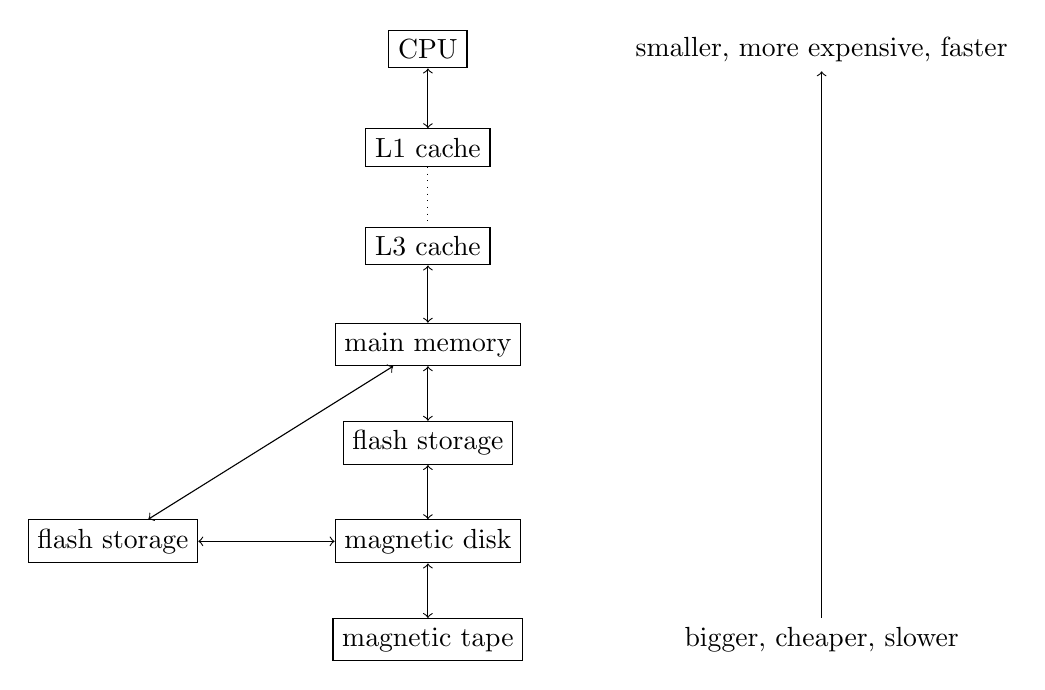
\begin{tikzpicture}[y=1.25cm]
                        \node[draw] (cpu) at (0, 0) {CPU};
                        \node[draw] (l1) at (0, -1) {L1 cache};
                        \node[draw] (l3) at (0, -2) {L3 cache};
                        \node[draw] (mm) at (0, -3) {main memory};
                        \node[draw] (fs1) at (0, -4) {flash storage};
                        \node[draw] (md) at (0, -5) {magnetic disk};
                        \node[draw] (fs2) at (-4, -5) {flash storage};
                        \node[draw] (mt) at (0, -6) {magnetic tape};

                        \draw
                        (cpu) edge[<->] (l1)
                        (l1) edge[dotted] (l3)
                        (l3) edge[<->] (mm)
                        (mm) edge[<->] (fs1)
                        (mm) edge[<->] (fs2)
                        (fs1) edge[<->] (md)
                        (fs2) edge[<->] (md)
                        (md) edge[<->] (mt);

                        \node (x) at (5, -6) {bigger, cheaper, slower};
                        \node (y) at (5, 0) {smaller, more expensive, faster};

                        \draw (x) edge[->] (y);
                    \end{tikzpicture}
                \end{center}
                Disks are still the main secondary storage device of choice, with the main advantage over tapes being the ability to perform random access, rather than purely sequential.
                Data is stored in units in \textbf{disk blocks} or \textbf{pages} (may be used interchangeably), typically in the order of kilobytes and occasionally megabytes.
                Unlike RAM, the time to retrieve / write a disk page varies depending on the location, with a tremendous impact on time to retrieve, hence relative placement of pages on a disk has a major impact on performance.
                The lecture then goes over the anatomy of a disk;
                \begin{itemize}
                    \itemsep0em
                    \item spindle and platters spin between 5,000 - 15,000 RPM (with physical limitations)
                    \item arm assembly has multiple disk head, one for each platter - the tracks under the heads form a cylinder
                    \item only one head reads or writes at once
                \end{itemize}
                The time to access a disk block has three elements;
                \begin{itemize}
                    \itemsep0em
                    \item \textbf{seek time} \hfill time to move the arm to the correct position (in and out, towards the spindle)
                    \item \textbf{rotational delay} \hfill arm assembly in a fixed position, block needs to be rotated under head
                    \item \textbf{transfer time} \hfill actual time to read data from disk into main memory
                \end{itemize}
                The time for a smaller number of cylinders traversed is dominated by the seek time (head positioning).
                In modern disks, short seeks are dominated by the \textbf{settle time}, which gets larger with increased disk track density.
                \medskip

                Generally, the seek time and rotational delay dominates, with the former being in the range of 1 to 20ms, and the latter being in the range of 0 to 10ms.
                On the other hand, the transfer rate is less than 1 millisecond for a 4KB page.
                As such, the key to lower I/O cost is to reduce the delays caused by seek and rotation.
                Additionally, in shared disks, most of the time is spent waiting for access to the arm.
                \medskip

                The concept of the next block is as follows;
                \begin{itemize}
                    \itemsep0em
                    \item blocks on the same track, followed by
                    \item blocks on the same cylinder
                    \item blocks on adjacent cylinder
                \end{itemize}
                We can't control where we write on the disk - that's controlled by the device driver.
                Typically, if data is written together, it will also be read together.
                Defragmentation is disk optimization, as data can be spread out all over a disk for a given file, leading to slower read times - this is done by putting all the pieces of a file closer together.
                \medskip

                Note that an adjacent block doesn't necessarily mean physically adjacent.
                Data can be physically spread out over a disk but in a certain pattern that can lead to near sequential access.
                The adjacent blocks can be the blocks under the disk head after rotating during settle time.
                \medskip

                In general, memory access is much faster than disk I/O (roughly $1,000 \times$), and sequential I/O is faster than random (roughly $10 \times$).
                \medskip

                The lowest layer of DBMS manages the space on the disk and higher levels can call this layer to allocate / de-allocate a page, or read / write a page.
            \subsubsection*{Summary}
                In general, the key for storing data on a disk is to store data together if it's queried together.
                Random access should be avoided, preferably use sequential access.
                Data structures should be aligned for page size - for example, if a data structure were to have a few bytes in the next page, an additional page would have to be retrieved, despite mostly being irrelevant.
        \subsection*{1.2 - Main Memory Indexing}
            The general trend is that we have more main memory as time goes on.
            The hardware trends show that CPU speed and main memory capacity doubles every 18 months, however memory speed only grows by 10\% per year.
            \medskip

            This means that many databases, typically OLTP, can fit into main memory; OLAP is still in the order of petabytes, if not more.
            Memory access has become the new bottleneck for main memory databases.
            There is no longer a uniform random access model (NUMA), meaning that we can no longer assume that accessing each piece of data in memory takes the same amount of time.
            Cache performance has become crucial.
            \medskip

            The memory hierarchy is as follows.
            Note that a cache \textbf{line} is the smallest unit that can be retrieved from the cache, and data structures should be aligned to a line in a similar way to pages.
            \begin{itemize}
                \itemsep0em
                \item CPU (registers)
                \item L1 cache, takes 1 cycle, 8-64 KB, 32 bytes per line
                \item L2 cache, takes 2 - 10 cycles, 64 - 128 bytes per line
                \item TLB, takes 10 - 100 cycles, 64 entries / pages
            \end{itemize}
            The cache performance is crucial, similar to the disk cache / buffer pool, however the DBMS doesn't have direct control of this.
            \subsubsection*{Improving Cache Performance}
                The primary factors are the cache capacity and data locality, the former is a given and can't be changed, whereas we can do something about the locality.
                An example with non-random access, such as a scan or index traversal is by clustering data structures to a multiple of a cache line, as well as squeezing more useful data into a cache line.
                On the other hand, with random access, such as in a hash join, the data should be partitioned to fit in cache / TLB.
                CPU is often also traded for memory access, such as compression (requires more CPU processing, but reduces storage usage).
            \subsubsection*{Trees}
                The lecture then goes through an example of a tree index, where each node holds 2 entries.
                Each node can point to three other nodes, where the values are either below, in between the two values, or higher than both.
                \medskip

                The B+ tree is quite similar, but all leaf nodes are connected.
                This allows for faster execution of range queries, as the nodes are connected without traversing up and down the tree.
                The \textbf{order} is the minimum number of keys or pointers in a non-leaf node and the \textbf{fanout} of a node is the number of pointers out of the node.
                These have the following properties;
                \begin{itemize}
                    \itemsep0em
                    \item balanced - leaves are at the same level, leading to predictable performance when traversing down the tree (same for every node)
                    \item every node, other than the root, must be at least half full meaning it becomes balanced
                    \item searching is $\log_d(n)$, where $d$ is the order and $n$ is the number of entries
                    \item insertion involves finding the leaf to insert to, splitting if the node is full and adjusting index accordingly; has a similar cost to searching, have to find all the way down, and may have to split all the way back up
                    \item deletion is similar, find leaf node, delete, and merge neighbouring nodes if required (not half-full)
                \end{itemize}
                \textbf{Cache sensitive search trees} can be thought of as a B+ tree that has been optimised specifically for main memory.
                The basic approach for this is to improve locality, with each node of the tree fitting into an L2 cache line, as the penalty of an L2 miss is significantly higher than that of an L1 miss, and can fit more nodes in L2 than L1.
                Keys are fixed length (from variable length) by the use of dictionary compression, letting us know the size of a child node.
                Child pointers are also eliminated; previously we had multiple pointers to point to each of the child nodes, however we now only need one pointer to a single child node as we know the size.
                \begin{center}
                    \begin{tikzpicture}
                        \begin{scope}[shift={(0, 0)}]
                            \begin{scope}[shift={(0, 0)}]
                                \node at (0, 0) {$2$};
                                \draw
                                (-1, -0.5) -- (1, -0.5) -- (1, 0.5) -- (-1, 0.5) -- cycle
                                (-0.5, -0.5) -- (-0.5, 0.5)
                                (0.5, -0.5) -- (0.5, 0.5);
                            \end{scope}
                            \begin{scope}[shift={(-1.5, -2)}]
                                \node at (0, 0) {$1$};
                                \draw
                                (-1, -0.5) -- (1, -0.5) -- (1, 0.5) -- (-1, 0.5) -- cycle
                                (-0.5, -0.5) -- (-0.5, 0.5)
                                (0.5, -0.5) -- (0.5, 0.5);
                            \end{scope}
                            \begin{scope}[shift={(1.5, -2)}]
                                \node at (0, 0) {$3$};
                                \draw
                                (-1, -0.5) -- (1, -0.5) -- (1, 0.5) -- (-1, 0.5) -- cycle
                                (-0.5, -0.5) -- (-0.5, 0.5)
                                (0.5, -0.5) -- (0.5, 0.5);
                            \end{scope}
                            \begin{scope}[shift={(-3, -4)}]
                                \node at (0, 0) {$1$};
                                \draw
                                (-0.5, -0.5) -- (1, -0.5) -- (1, 0.5) -- (-0.5, 0.5) -- cycle
                                (0.5, -0.5) -- (0.5, 0.5);
                            \end{scope}
                            \begin{scope}[shift={(-1, -4)}]
                                \node at (0, 0) {$2$};
                                \draw
                                (-0.5, -0.5) -- (1, -0.5) -- (1, 0.5) -- (-0.5, 0.5) -- cycle
                                (0.5, -0.5) -- (0.5, 0.5);
                            \end{scope}
                            \begin{scope}[shift={(1, -4)}]
                                \node at (0, 0) {$3$};
                                \draw
                                (-0.5, -0.5) -- (1, -0.5) -- (1, 0.5) -- (-0.5, 0.5) -- cycle
                                (0.5, -0.5) -- (0.5, 0.5);
                            \end{scope}
                            \begin{scope}[shift={(3, -4)}]
                                \node at (0, 0) {$4$};
                                \draw
                                (-0.5, -0.5) -- (1, -0.5) -- (1, 0.5) -- (-0.5, 0.5) -- cycle
                                (0.5, -0.5) -- (0.5, 0.5);
                            \end{scope}

                            \draw
                            (-0.75, 0) edge[->] (-1.5, -1.5)
                            (0.75, 0) edge[->] (1.5, -1.5)
                            (-2.25, -2) edge[->] (-3, -3.5)
                            (-0.75, -2) edge[->] (-1, -3.5)
                            (0.75, -2) edge[->] (1, -3.5)
                            (2.25, -2) edge[->] (3, -3.5)
                            (-2.25, -4) edge[->] (-2.25, -5)
                            (-0.25, -4) edge[->] (-0.25, -5)
                            (1.75, -4) edge[->] (1.75, -5)
                            (3.75, -4) edge[->] (3.75, -5);
                        \end{scope}

                        \begin{scope}[shift=({10, 0})]
                            \draw
                            (-1.5, 0.5) -- (1.5, 0.5) -- (1.5, -0.5) -- (-1.5, -0.5) -- cycle
                            (-0.5, 0.5) -- (-0.5, -0.5)
                            (0.5, 0.5) -- (0.5, -0.5);
                            \node at (-1, 0) {$1$};
                            \node at (0, 0) {$2$};
                            \node at (1, 0) {$3$};

                            \begin{scope}[shift={(-3, -4)}]
                                \node at (0, 0) {$1$};
                                \draw
                                (-0.5, -0.5) -- (1, -0.5) -- (1, 0.5) -- (-0.5, 0.5) -- cycle
                                (0.5, -0.5) -- (0.5, 0.5);
                            \end{scope}
                            \begin{scope}[shift={(-1, -4)}]
                                \node at (0, 0) {$2$};
                                \draw
                                (-0.5, -0.5) -- (1, -0.5) -- (1, 0.5) -- (-0.5, 0.5) -- cycle
                                (0.5, -0.5) -- (0.5, 0.5);
                            \end{scope}
                            \begin{scope}[shift={(1, -4)}]
                                \node at (0, 0) {$3$};
                                \draw
                                (-0.5, -0.5) -- (1, -0.5) -- (1, 0.5) -- (-0.5, 0.5) -- cycle
                                (0.5, -0.5) -- (0.5, 0.5);
                            \end{scope}
                            \begin{scope}[shift={(3, -4)}]
                                \node at (0, 0) {$4$};
                                \draw
                                (-0.5, -0.5) -- (1, -0.5) -- (1, 0.5) -- (-0.5, 0.5) -- cycle
                                (0.5, -0.5) -- (0.5, 0.5);
                            \end{scope}

                            \draw
                            (-1.5, -0.5) edge[dotted, ->] (-3, -3.5)
                            (-0.5, -0.5) edge[dotted, ->] (-1, -3.5)
                            (0.5, -0.5) edge[dotted, ->] (1, -3.5)
                            (1.5, -0.5) edge[dotted, ->] (3, -3.5)
                            (-2.25, -4) edge[->] (-2.25, -5)
                            (-0.25, -4) edge[->] (-0.25, -5)
                            (1.75, -4) edge[->] (1.75, -5)
                            (3.75, -4) edge[->] (3.75, -5);
                        \end{scope}
                    \end{tikzpicture}
                \end{center}
                In the example above, we assume a cache line size of 24 bytes, a key size (and pointer size) of 4 bytes.
                The B+ tree on the left is 2-way, with 3 misses, and the CSS tree is 4-way, with only 2 misses.
                \medskip

                CSS has the best search / space balance; second best search to hash, which has poor space, and also second best space to binary search, which has poor search.
                The space taken is roughly half that of a B+ tree.
                However, this cannot support dynamic updates as the fan-out and array size must both be fixed.
                \medskip

                A \textbf{CSB+} tree addresses this.
                Children of the same node are stored in an array / node group and the parent only has a single pointer to the child array.
                This has a similar search performance to the CSS tree, and has good update performance if no split occurs.
                Splits are still required as we still have a maximum capacity of an array, which requires allocating new memory.
                \medskip

                A variant of this is a CSB+ tree with segments; the child array is divided into segments, typically 2, with one child pointer per segment.
                This improves split performance, but worsens search performance.
                Another variant is a full CSB+ tree, which is a CSB+ tree with a pre-allocated children array, obviously requiring more space but is good for search and insertion (no more memory needs to be allocated, as it's all allocated).
                It's important to note that none of these are as \textbf{flexible} as B+ trees, but perfectly fine for certain workloads.
                \medskip

                The general performance is as follows, for search, CSS is fastest, followed by full CSB+ (joined with CSB+), then followed by CSB+ with segments, and finally B+.
                On the other hand, with insertion, B+ has the best, roughly equal to full CSB+, which is followed by CSB+ with segments, then CSB+, and finally CSS.
                Generally, full CSB+ is ideal if space isn't a concern, CSB+ (and with segments) is ideal if there are more reads than insertions, and finally CSS is best when read-only.
            \subsubsection*{Cache Conscious Join Method}
                Typically, in vertical decomposed storage, what we want to do when we join in main memory is to partition a base table into $m$ arrays, where $m$ is the number of attributes.
                Variable length fields should also be converted to fixed length fields via the use of dictionary compression.
                For example;
                \begin{center}
                    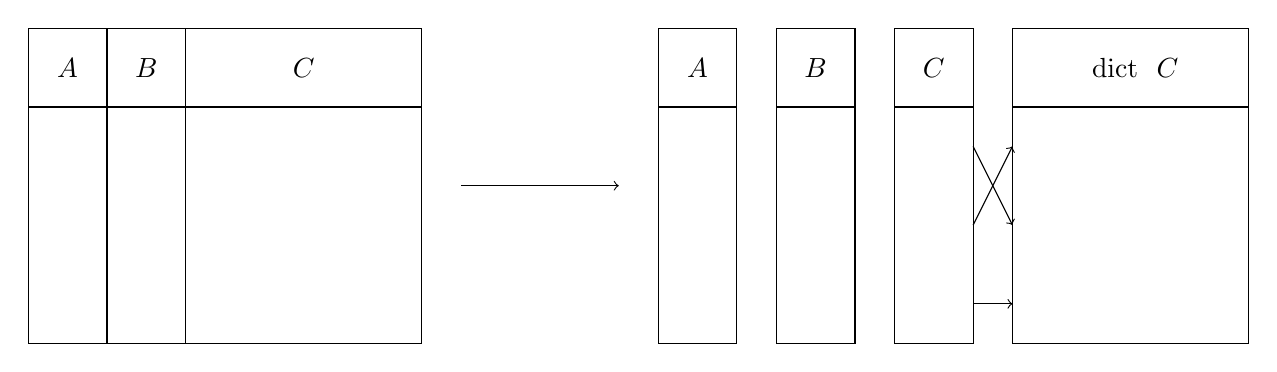
\begin{tikzpicture}[x=0.5cm]
                        \draw
                        (0, 0) -- (10, 0) -- (10, -4) -- (0, -4) -- cycle
                        (0, -1) -- (10, -1)
                        (2, 0) -- (2, -4)
                        (4, 0) -- (4, -4);
                        \node at (1, -0.5) {$A$};
                        \node at (3, -0.5) {$B$};
                        \node at (7, -0.5) {$C$};

                        \draw (11, -2) edge[->] (15, -2);
                        \draw
                        (16, 0) -- (18, 0) -- (18, -4) -- (16, -4) -- cycle
                        (16, -1) -- (18, -1)
                        (19, 0) -- (21, 0) -- (21, -4) -- (19, -4) -- cycle
                        (19, -1) -- (21, -1)
                        (22, 0) -- (24, 0) -- (24, -4) -- (22, -4) -- cycle
                        (22, -1) -- (24, -1)
                        (25, 0) -- (31, 0) -- (31, -4) -- (25, -4) -- cycle
                        (25, -1) -- (31, -1)
                        (24, -1.5) edge[->] (25, -2.5)
                        (24, -2.5) edge[->] (25, -1.5)
                        (24, -3.5) edge[->] (25, -3.5);
                        \node at (17, -0.5) {$A$};
                        \node at (20, -0.5) {$B$};
                        \node at (23, -0.5) {$C$};
                        \node at (28, -0.5) {~dict~ $C$};
                    \end{tikzpicture}
                \end{center}
                Each array contains a pair of OID (uniquely identifies an entry) and value for the $i^\text{th}$ attribute.
                Reconstruction is a simple array access in this case.
                Joins are much more efficient, as we no longer have to read all the data.
                \medskip

                The existing equal-join methods;
                \begin{itemize}
                    \itemsep0em
                    \item sort-merge
                        \subitem one of the relations will not fit in cache, likely meaning we have to read into cache multiple times (take smaller of two relations in main memory)
                    \item hash join \hfill bad if the inner relation doesn't fit into cache
                    \item clustered hash join
                        \subitem one pass to generate cache-sized partitions, take each partition and join it with the other relation, and so on, best of the three solutions, but can be bad if the number of partitions exceed the number of cache lines / TLB entries - can lead to cache thrashing
                \end{itemize}
                This can be addressed with \textbf{radix join}, which first partitions one of the relations and ensure that we partition it into partitions such that we have matching partitions based on $B$ bits of the attribute.
                Matching partitions are joined, nested-loop can be done for small ($\leq 8$ tuples) partitions or a hash join for larger partitions, which is $\leq$ L1 cache, L2 cache, or TLB size (with L1 being ideal).
                This avoids thrashing, compared to clustered hash join.
                Saving these cache misses outweighs the cost of performing extra partitions.
            \subsubsection*{Conclusion}
                The cache performance is important and will become more important as main memory grows.
                The key to this is to cluster data (into a cache line); data that is read together should be written and stored together.
                Irrelevant data should be omitted, including pointers and the use of vertical decomposition.
                Partitions should be done to avoid thrashing.
            \subsubsection*{Spatial Data}
                Spatial data is data with any three dimensions; such as points.
                It has queries such as range queries, nearest neighbours, etc.
                Objects near each other should be stored on the same disk page / cache line, however, there isn't an ordering on data in three dimensions (two objects that are close in 1 dimension could be far apart in another).
                \medskip

                This then goes over an example with reducing computation.
                In the example, checking a range on non-uniform (spatial) partitioning is expensive, as there are many irrelevant points.
                The computation is reduced by using several grids of varying detail; if the range covers the majority of a cell it's checked on that level of detail, if not, it's checked on a lower level of detail.
        \subsection*{October 14 - Live Lecture}
            Learned indexing combines machine learning with indexing.
            The same concept of an index applies, but machine learning models aid to accelerate this lookup, for example by learning distributions.
            These models are typically small and simple, such as interpolation - however, they understand distributions better than existing structures such as B trees.
            The primary challenge is that these models need to fit into main memory, or even the cache to be faster.
            \medskip

            The fundamental problem of a join is to join two relations on a shared attribute.
            If one of the iterations is small, you can iterate over the smaller relation and lookup the related element in the larger relation.
            There are typically two phases in a join, with a build (scanning through the smaller relation and building a hash table), and a probe phase where the second input relation is scanned, and the hash table of the first relation is probed for the matching tuple.
            The problem with this is when the hash table is large, leading to a large number of cache misses.
            One solution is to ensure the hash table can be broken into chunks that fit into cache.
            However, if there are too many partitions, the build phase involves many writes into different partitions, leading to many writes into different locations (thus leading to many TLB misses).
            The radix join addresses this by iteratively partitioning into cache. % ?
            \medskip

            The data in a B+ tree exists in the leaves.
            Any other numbers in internal nodes only exist to help guide the search.
            \medskip

            An adjacent block doesn't necessarily mean a short / small seek distance.
            The abstract concept of an adjacent block could also be called a temporally close block; could be short seek distance or based on rotation.
            Note that the platter is rotating constantly, and by the time the head has finished moving, a different block would be under the head, not necessarily one that is physically nearby.
            If data is written together, it will be stored on adjacent (the abstract concept) blocks, which may still be spread over the disk physically.
            \medskip

            When there's indexing in main memory, the performance is so much faster, the index needs much fewer instructions, otherwise it may be faster to just scan.
            On the other hand, on disks, the performance is relatively slower, allowing for more complex indices.
            This applies even for high-throughput devices.
            \medskip

            DBMS doesn't typically bypass the OS, at least not without a custom OS or specific hardware.
            However, it organises its files or data separately, not leaving it to the OS, as well as handling its own cache and database pages (managed by the database system itself).
            Typically, database systems stores the data in and builds on the OS filesystem.
            You can't force the disk to read / write in a specific physical location, but you can help it write in one go.
        \subsection*{2.1 - Solid State Storage}
            Flash disks can be used as secondary storage or as a caching layer, with the main advantage over traditional disks being that random reads are as fast as sequential reads.
            Disadvantages are slower random writes and a limited number of write cycles.
            Data is organised in pages, which is organised in \textbf{flash blocks}.
            Similar to RAM, the time to retrieve a page isn't related to the location.
            The internals of a flash package are as follows;
            \begin{center}
                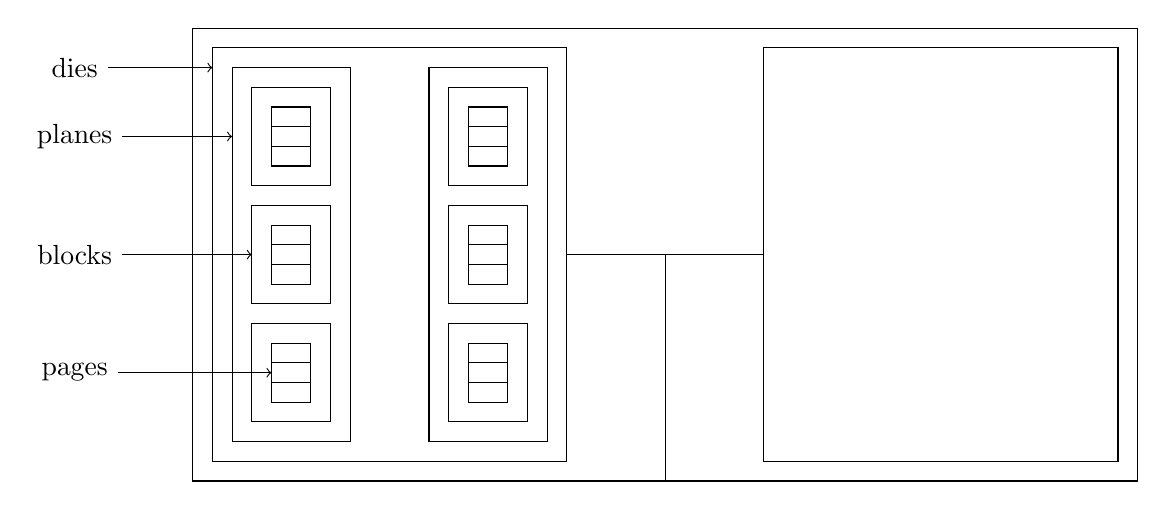
\begin{tikzpicture}[x=0.25cm, y=0.25cm]
                    \node (d) at (-10, 2) {dies};
                    \node (pl) at (-10, -1.5) {planes};
                    \node (b) at (-10, -7.5) {blocks};
                    \node (pa) at (-10, -13.5) {pages};

                    \draw
                    (d) edge[->] (-3, 2)
                    (pl) edge[->] (-2, -1.5)
                    (b) edge[->] (-1, -7.5)
                    (pa) edge[->] (0, -13.5);

                    \draw
                    (-4, 4) -- (44, 4) -- (44, -19) -- (-4, -19) -- cycle
                    (-3, 3) -- (15, 3) -- (15, -18) -- (-3, -18) -- cycle
                    (25, 3) -- (43, 3) -- (43, -18) -- (25, -18) -- cycle
                    (15, -7.5) -- (25, -7.5)
                    (20, -7.5) -- (20, -19);
                    \foreach \x in {0, 10} {
                        \begin{scope}[shift={(\x, 0)}]
                            \draw (-2, 2) -- (4, 2) -- (4, -17) -- (-2, -17) -- cycle;
                            \foreach \y in {0, -6, -12} {
                                \begin{scope}[shift={(0, \y)}]
                                    \draw
                                    (-1, 1) -- (3, 1) -- (3, -4) -- (-1, -4) -- cycle
                                    (0, 0) -- (2, 0) -- (2, -3) -- (0, -3) -- cycle
                                    (0, -1) -- (2, -1)
                                    (0, -2) -- (2, -2);
                                \end{scope}
                            };
                        \end{scope}
                    };
                \end{tikzpicture}
            \end{center}
            There are many of these within an SSD, which in turn is structured as an interface (either SATA or PCI) connected to the internal CPU which is connected to internal memory and the flash controller, which is connected to many flash packages.
            There are no moving parts, hence no mechanical limitations.
            The flash controller helps to ensure the entire drive degrades at roughly the same rate (wear levelling), preventing the capacity from shrinking.
            The access time depends on the bandwidth of the flash packages, device organisation as well as software efficiency.
            The flash translation layer (FTL) is the firmware that manages the hardware.
            \medskip

            A write involves copying the page we are writing to a new page and then deleting the old page, leading to slower random writes.
            On the other hand, if we do a serial write, we can keep it in memory until we have a full flash page.
            Deletion takes time (and is typically on the block level, rather than page) as the pages are densely packed and a high voltage is required to erase a page, seeping into other pages.
            Blocks are isolated from each other, but pages are not (would waste space).
            \medskip

            As the latency gap between CPU and RAM grew, caches were introduced to bridge the gap.
            Similarly, the gap between RAM and HDD can be bridged with SSMs (solid state memory) as a cache or buffer.
            \medskip

            Today, only flash and PCM (phase change memory) are pursued commercially.
            PCM could be placed below flash in the memory hierarchy as the density is still too low.
            \medskip

            DBMS is traditionally designed around a HDD model (buffer management, etc).
            Transactions are only really there (ACID properties) as we need to run things in parallel (since we're waiting on disk and don't want to block).
            Similarly, query plans are also HDD optimisations in the sense they prefer sequential over random access.
            \medskip

            Flash can either be used to replace HDDs, act as an intermediate layer between HDD and RAM, or be used with HDDs on the same level.
            The correct use depends on the workload, such as the amount of data or how the data is accessed, as well as future trends in terms of density.
            \medskip

            Some uses of SSDs in databases;
            \begin{enumerate}[1.]
                \itemsep0em
                \item \textbf{flash-only OLTP}
                    \smallskip

                    OLTP is dominated by random reads and writes, which is very bad for disks, but much faster on flash.
                    With random writes, when used naively in place of a HDD, the throughput drops substantially over time, with significant variance.
                    \medskip

                    The append / pack algorithm; for an append-only operation, we write sequentially as much as we can.
                    No updates are done in place, but rather the old page is invalidated (after reading the content) and a new page is written.
                    Once we run out of space, we reclaim the space and reorganise the storage and continue to write the pages in append-only.
                    Essentially, random writes are transformed into sequential writes and a garbage collection step takes place (with some overhead).
                    This adapts the properties of the algorithm to the underlying hardware.
                \item \textbf{flash-aided business intelligence (OLAP)}
                    \smallskip

                    These are typically read-only queries, with very few scattered updates and complex queries.
                    There are typically two choices - for freshness, updates are performed in-place (with the queries), whereas for performance, updates are done in batches (separate from queries).
                    However, there may be stale data in the latter case.
                    \medskip

                    Flash can be used as a write cache for analytics.
                    Incoming data is written to the SSD, which is then merged with data from the disks to answer a query.
                    We are only using SSDs where it's beneficial; for random accesses.
                    This essentially buffers updates on flash rather than memory, which is larger, cheaper, and also persistent.
                    Of course, this comes with limitations including avoiding random writes (which we saw how to overcome earlier), as well as a limited number of writes due to endurance issues.
                    \medskip

                    The concept behind \textbf{Materialised Sort-Merge (MaSM)} is that we have a system for large scans of tables (like OLAP) which keeps the data on disk when it does it well, but puts updates (where the performance is poor) on SSDs.
                    The data is then merged when queried.
                \item \textbf{logging on flash + HDD}
                    \smallskip

                    Transaction logging is a major bottleneck.
                    Logs are typically what transactions are to be executed (so it can be redone on a failure), which are small sequential writes.
                    The access pattern for this involves small sequential writes which causes a HDD to incur rotational delays.
            \end{enumerate}
            In general, they can be used as a helper on the memory level (not changing the DBMS), adapt the I/O pattern with small DBMS changes, or to fully change storage management.
        \subsection*{2.2 - In-Memory Databases}
            OLAP deals with large amounts of data (data warehousing / data mining) where we look at the output of operational databases, turn them into historical databases and run large, complex, aggregation queries.
            The queries are long running and deal with a large number of tables, and are mostly read-only (only analysing the business).
            On the other hand, OLTP are primarily transactions, hence many small updates.
            There are very few tables touched, with generated queries (not typically human-written).
            \medskip

            OLAP databases are in the order of petabytes, which need to be stored on disks or similar.
            On the other hand, transactional databases are quite small and not growing much; it's possible to buy a TB of main memory.
            \medskip

            On the \textit{Shore DBMS} prototype, only 4\% of the CPU cycles are spent on actual useful work, whereas the remaining 96\% are spent (equally) on latching, recovery (dealing with the log file), locking, and the buffer pool (reading and writing between main memory and disk).
            To improve the performance, improving overhead in processing (better data structures etc., only improves 4\% of the actual performance).
            However, deploying in main memory gets rid of the buffer pool entirely, leading to a solid improvement in performance.
            \medskip

            We have three choices of solutions;
            \begin{itemize}
                \itemsep0em
                \item \textbf{OldSQL} \hfill legacy RDBMS
                    \smallskip

                    Traditional SQL doesn't scale well in the distributed sense.
                \item \textbf{NoSQL} \hfill give up ACID properties to accelerate performance
                    \smallskip

                    ACID properties and transactions are difficult to scale out.
                    Also gives up SQL; the SQL is translated at compile time to a sequence of low level operations (difficult to do).
                    High level queries are also good for abstraction.
                    Giving up data consistency can also be a big issue with NoSQL.
                    \medskip

                    This is appropriate for non-transactional systems, without shared state, and single record transactions that are commutative.
                \item \textbf{NewSQL} \hfill preserves SQL and ACID
                    \smallskip

                    This has both SQL and ACID, and performance and scalability is provided through modern software architecture.
                    It requires solutions for the following, all of which are large sources of overhead;
                    \begin{itemize}
                        \itemsep0em
                        \item \textbf{traditional record level locking} \hfill timestamp order
                        \item \textbf{buffer pool overhead} \hfill removed when moved to main memory
                        \item \textbf{latching for shared data structures} \hfill single-threading for small operations
                        \item \textbf{write-ahead logging} \hfill how to address failure
                    \end{itemize}
            \end{itemize}
            The example we're going to use for NewSQL is \textit{VoltDB}.
            It's all in main-memory (no buffer pool), small single threaded transaction (no concurrency, hence no locks or latches required), and has durability and availability through copies (redundancy) - therefore no traditional log is required.
            Now the 95\% of the cycles are for useful work (with the remainder still being used for some locking).
            \textit{VoltDB} currently runs a subset of SQL, on clusters with LAN and WAN replication.
            It can scale to 384 cores.
            The only locking involved is for multi-partition operations.
            \medskip

            For each of the solutions, only NewSQL is suitable for new OLTP;
            \begin{itemize}
                \itemsep0em
                \item OldSQL is too slow and doesn't scale
                \item NoSQL lacks consistency guarantees and has no language to express queries on a high level (difficult to use)
                \item NewSQL is fast, scalable, consistent, and supports a high level language
            \end{itemize}
            There is a partition per physical CPU core, hence each physical server typically has multiple \textit{VoltDB} partitions.
            Tables can either be \textbf{partitioned} or \textbf{replicated}.
            The former has a single column acting as the partitioning key, allowing rows to be spread across all partitions by the partition column.
            This is better for data with a high modification frequency (transactional data) as it reduces the amount of data being touched.
            On the other hand, the latter has all rows existing in \textbf{all} partitions and is better for mostly static data.
            \medskip

            Similarly, there are also two types of work, which are both ACID.
            Single-partition work happens within a single partition (and requires no locking as it's in a single thread) and is more suitable for the majority of transactional work.
            On the other hand, multi-partition work where we have queries that touch multiple partitions.
            \medskip

            Consider the following ``schema'', where we have three partitions (customer IDs 1 and 4 are in partition 1, 2 and 5 in partition 2, and 3 and 6 in partition 3);
            \begin{lstlisting}
                table orders (partitioned):
                    customer_id (partition key)
                    order_id
                    product_id

                table products (replicated):
                    product_id
                    product_name
            \end{lstlisting}
            Examples of queries are;
            \begin{itemize}
                \itemsep0em
                \item ~select count(*) from orders where customer\_id = 5~ \hfill single (p2)
                \item ~select count(*) from orders where product\_id = 3~ \hfill multi
                    \subitem multi-partition as we don't partition on ~product\_id~, however it's a read operation and no locking is required
                \item ~insert into orders (customer\_id, order\_id, product\_id) values (3,302,2)~ \hfill single (p3)
                    \subitem single-partition if all the values fit in the same partition
                \item ~update products set product\_name = 'spork' where product\_id = 3~ \hfill multi
                    \subitem updating replicated data requires some locking
            \end{itemize}
            In each partition there is a work queue where the queries are coming in.
            There is data for the table and the indices, and a single execution engine which executes requests sequentially - once again, no locking is required as there is no parallelism.
            \medskip

            The database is constructed from the schema (DDL), the work (Java stored procedures), and the project containing users, groups, and partitioning.
            The \textit{VoltCompiler} creates an application catalogue distributed to all machines.
            All access is via Java stored procedures, a single invocation is a transaction that is committed on success, limiting round trips between the DB and the application.
            Communication with the client is asynchronous.
            \medskip

            This scales by adding more machines (or more RAM for more main memory).
            There is high availability from K-safety for redundancy, and snapshots are available, either scheduled, continuous, or on demand (which can be spooled to a data warehouse).
            \medskip

            Due to the asynchronous calls, invocations are sent and responses are pulled from the server, allowing a single client to generate more than 100K transactions per second (TPS) - the client will behave synchronously if required.
            \begin{lstlisting}
                traditional:
                  salary = get_salary(employee_id);
                VoltDB:
                  callProcedure(asyncCallback, "get_salary", employee_id);
            \end{lstlisting}
            However, it doesn't support client-side transaction control (the client cannot perform a rollback) - a stored procedure will commit if it's successful and rollback otherwise.
            The procedure can can call for rollback.
            \medskip

            The lack of concurrency can be beneficial, but it's also important to ensure that any single query is short (transactions should execute in microseconds).
            `Inventory' type applications benefit from this.
            Since locking doesn't have to be considered, dead-locks aren't a concern either.
            As other transactions wait for the running transaction to complete, nothing intensive should be done in a stored procedure (requesting web pages, etc.) - this is useful for OLTP but not OLAP.
            This is optimised for throughput, not latency.
            \medskip

            A subset of SQL is supported; ~SELECT~, ~INSERT~ (with values), ~UPDATE~, and ~DELETE~.
            Aggregations such as ~AVG~, ~COUNT~, ~MAX~, ~MIN~, and ~SUM~ are also supported.
            Functionality will be added over time, but can be done in Java already.
            The execution plan is created at compile time (can be analysed), but may lead to performance issues if there's a drastic change to the cardinality of data (recompile and redeploy in this case)
        \subsection*{October 18 - Live Lecture}
            With SSDs, each page has a limited number of write cycles (around 3,000 per page).
            However, we cannot write to a specific page directly anyways, as this abstracted away by the firmware.
            One important thing to keep in mind is that due to this limitation on SSDs, there may be issues when replacing a HDD for a write-heavy workload.
            Wear-levelling attempts to spread the writes evenly (as much as possible).
            To minimise writes, we should pack writes to be in the sizes of pages.
            When we scan (read sequentially), we are typically limited by the bandwidth of the connection rather than the devices.
            \medskip

            The need for transactions comes from the use of concurrency, which is in place to keep the CPU busy (in traditional databases).
            However, this is not a concern in \textit{VoltDB} as operations are done in serial.
            Locks are to separate user transactions (and protects database contents during entire transactions) and latches are used to separate threads (and protects in-memory data structures during critical sections).
            \medskip

            A concrete example for a fine-grained index versus a coarse-grained one is as follows.
            The former would index every element of an array whereas the latter could take a bunch of entries and index on that; once you're in the `bunch', you still have to perform a scan within it.
            This reduces the complexity by reducing the number of items indexed.
            \medskip

            While \textit{VoltDB} could be constrained by the network bandwidth, however it would likely not reach a bottleneck as the operations are very small (OLTP).
            Additionally, we can't increase transactions indefinitely as it still takes time to process (CPU would be overwhelmed first).
            \medskip

            Append-pack requires more space on the SSD as there is redundant data.
            There is garbage collection to run over the data and pack it together, similar to how defragmentation works.
            There will be some extra work to do (to check whether the page is valid), however overall it's fast enough.
        \subsection*{3 - Graph Databases}
            The example in this lecture will use \textit{Neo4j}, other examples include \textit{OrientDB}, \textit{InfiniteGraph}, and \textit{AllegroGraph}.
            A graph database is a fundamentally different model from traditional relational databases, where we have nodes and relationships between the nodes.
            \medskip

            Graph databases are fairly powerful (and as general as RDBMS, with a fairly direct correspondence between them for translation).
            Works very well if they fit in the main memory of the machine.
            Graph queries check which nodes are connected together.
            Additionally, it's easy to query and scales well on one machine.
            However, scaling out (to multiple machines) is quite difficult - we have graph queries that query relationships between nodes, however this may lead to querying different machines.
            \medskip

            A graph is an abstract representation of a set of objects, with pairs of these objects (also known as vertices or nodes) connected by links (also referred to as edges, arcs, or relationships).
            The different types of graphs are as follows;
            \begin{itemize}
                \itemsep0em
                \item \textbf{undirected} \hfill no indication of direction
                    \begin{center}
                        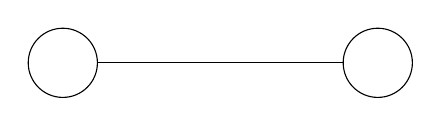
\begin{tikzpicture}
                            \node[state] (a) at (0, 0) {};
                            \node[state] (b) at (4, 0) {};
                            \draw (a) -- (b);
                        \end{tikzpicture}
                    \end{center}
                \item \textbf{directed} \hfill indication of direction, obviously
                    \begin{center}
                        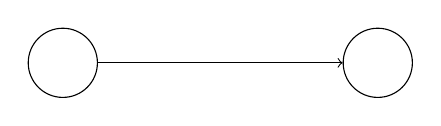
\begin{tikzpicture}
                            \node[state] (a) at (0, 0) {};
                            \node[state] (b) at (4, 0) {};
                            \draw (a) edge[->] (b);
                        \end{tikzpicture}
                    \end{center}
                \item \textbf{pseudo} \hfill only one relationship, pointing to itself
                    \begin{center}
                        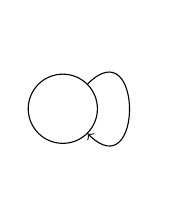
\begin{tikzpicture}
                            \node[state] (a) at (0, 0) {};
                            \draw (a) edge[->, loop, out=45, in=-45, distance=1cm] (a);
                        \end{tikzpicture}
                    \end{center}
                \item \textbf{multi} \hfill multiple relationships between nodes
                    \begin{center}
                        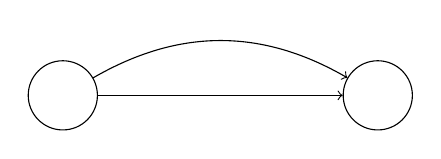
\begin{tikzpicture}
                            \node[state] (a) at (0, 0) {};
                            \node[state] (b) at (4, 0) {};
                            \draw
                            (a) edge[->] (b)
                            (a) edge[->, bend left=30] (b);
                        \end{tikzpicture}
                    \end{center}
                \item \textbf{hyper} \hfill multiple outgoing relationships
                    \begin{center}
                        \begin{tikzpicture}
                            \node[state] (a) at (0, 0) {};
                            \node[state] (b0) at (4, 2) {};
                            \node[state] (b1) at (4, 0) {};
                            \node[state] (b2) at (4, -2) {};
                            \draw
                            (a) edge[->] (b0)
                            (a) edge[->] (b1)
                            (a) edge[->] (b2);
                        \end{tikzpicture}
                    \end{center}
                \item \textbf{weighted} \hfill associated weight with the relationship
                    \begin{center}
                        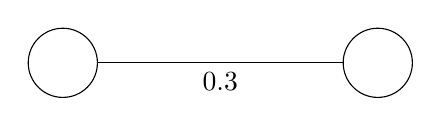
\begin{tikzpicture}
                            \node[state] (a) at (0, 0) {};
                            \node[state] (b) at (4, 0) {};
                            \draw (a) edge[below] node{$0.3$} (b);
                        \end{tikzpicture}
                    \end{center}
                \item \textbf{labelled} \hfill labels for nodes and relationships
                    \begin{center}
                        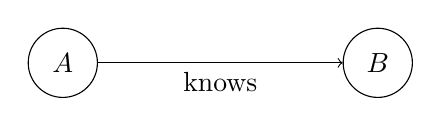
\begin{tikzpicture}
                            \node[state] (a) at (0, 0) {$A$};
                            \node[state] (b) at (4, 0) {$B$};
                            \draw (a) edge[->, below] node{knows} (b);
                        \end{tikzpicture}
                    \end{center}
                \item \textbf{property}
                    \begin{center}
                        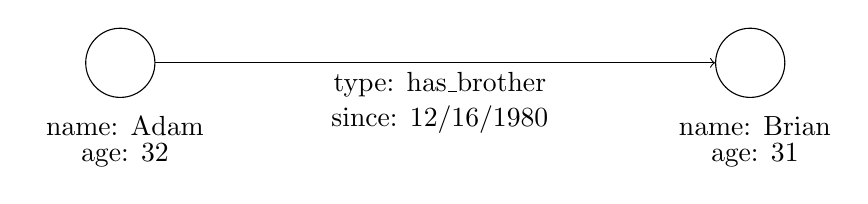
\begin{tikzpicture}
                            \node[state] (a) at (0, 0) {};
                            \node[state] (b) at (8, 0) {};
                            \draw (a) edge[->, below] node{\shortstack{~type: has\_brother~\\~since: 12/16/1980~}} (b);
                            \node at (0, -1) {\shortstack{~name: Adam~\\~age: 32~}};
                            \node at (8, -1) {\shortstack{~name: Brian~\\~age: 31~}};
                        \end{tikzpicture}
                    \end{center}
                    This is the closest to what \textit{Neo4j} uses.
                    In this property graphs, nodes and relationships can have arbitrary properties, typically key-value pairs.
            \end{itemize}
            Consider a many-to-many relationship in a typical RDBMS, in this example we have ~people~, ~departments~, and ~department\_member~ tables (where the latter joins the former two).
            In a graph model, there could simply be relationships from each entry in ~people~ to each of the entries in ~department~, with a ~belongs\_to~ (or similar) relationship.
            This eliminates the requirement for joins, which can be complicated if many joins are involved.
            A graph data model can be easily constructed by writing down the entities involved as nodes and then creating relationships between them.
            From here, properties (key-value pairs) can be added in to the nodes and relationships.
            It's generally quite similar to ER mapping, but we don't need to consider cardinality.
            \medskip

            A graph databases has an explicit graph structure, with each node knowing its adjacent nodes (has links to) - which ideally lives in the same machine.
            Each node has indices for its neighbouring nodes to allow for fast access; the cost for a local step remains the same even if the number of nodes increase, however it can become slower if the hops are to different machines (network latency).
            \medskip

            To translate to \textit{Neo4j};
            \begin{itemize}
                \itemsep0em
                \item each entity table is a label on nodes
                \item each row in an entity table is a node, with the columns being node properties
                \item add unique constraints for business primary keys and indices for attributes which are frequently looked up
            \end{itemize}
            A node can have relationships and properties.
            A relationship has a start and end node, has a relationship type which is uniquely identified by a name, and can have properties.
            Property keys are strings, whereas property values can either be a primitive type or an array of a primitive type.
            A path in \textit{Neo4j} is one or more nodes with connection relationships that can be retrieved as a query or the result of a traversal.
            Querying this in a traditional relational database could be very inefficient as you may end up querying tables multiple times.
            \medskip

            Cypher is very similar to SQL, but for graphs.
            It is a declarative (no need to tell it how to retrieve things), pattern-matching language.
            Some examples are as follows;
            \begin{itemize}
                \itemsep0em
                \item retrieves all pairs of nodes that are connected with a relationship; doesn't specify \textbf{what} relationship
                    \begin{lstlisting}
                        START a=node(*) // now optional
                        MATCH (a)-->(b) // a and b are just placeholders (connection is important)
                        RETURN a, b;
                    \end{lstlisting}
                \item find all nodes with an outgoing relationship and get a specific property (~name~ in this case) - no set property schema (similar to document databases), just ensure no name collisions
                    \begin{lstlisting}
                        START a=node(*)
                        MATCH (a)-->()
                        RETURN a.name;
                    \end{lstlisting}
                \item find all actors which have acted in a movie
                    \begin{lstlisting}
                        START a=node(*)
                        MATCH (a)-[:ACTED_IN]->(m)
                        RETURN a, m;
                    \end{lstlisting}
                \item with paths, note that ~(a)-->(b)-->(c)~ is different from ~(a)-->(b)<--(c)~
                \item get actor and director names for movie titles;
                    \begin{lstlisting}
                        START a=node(*)
                        MATCH (a)-[:ACTED_IN]->(m)<-[:DIRECTED]-(d)
                        // equivalent to the following (since m is named);
                        // MATCH (a)-[:ACTED_IN]->(m), (m)<-[:DIRECTED]-(d)
                        // MATCH (a)-[:ACTED_IN]->(m), (d)-[:DIRECTED]->(m)
                        RETURN a.name, m.title, d.name;
                    \end{lstlisting}
                \item sorting and limit can also be done (same as SQL) (count movies actors and directors have worked together in);
                    \begin{lstlisting}
                        START a=node(*)
                        MATCH (a)-[:ACTED_IN]->(m)<-[:DIRECTED]-(d)
                        RETURN a.name, d.name, count(*) AS count
                        ORDER BY(count) DESC
                        LIMIT 5;
                    \end{lstlisting}
                \item aggregations
                    Aggregations can also be done in a similar way;
                    \begin{itemize}
                        \itemsep0em
                        \item ~count(x)~ \hfill add number of occurrences
                        \item ~min(x)~ \hfill get lowest value
                        \item ~max(x)~ \hfill get highest value
                        \item ~avg(x)~ \hfill average of numeric values
                        \item ~collect(x)~ \hfill collects into an array (`transposes' a column)
                    \end{itemize}
                    An example of this is as follows, where we get the actors and directors who have worked together (and an array of movie titles);
                    \begin{lstlisting}
                        START a=node(*)
                        MATCH (a)-[:ACTED_IN]->(m)<-[:DIRECTED]-(d)
                        RETURN a.name, d.name, collect(m.title);
                    \end{lstlisting}
                \item find a specific node (query all nodes); in this example we search for the name ~John Smith~
                    \begin{lstlisting}
                        START n=node(*)
                        WHERE has(n.name) AND n.name = "John Smith"
                        RETURN n;
                    \end{lstlisting}
                    Note that the ~has(n.name)~ part ensures that the ~name~ property exists.
                    This is required as we don't know that every node has this property.
                \item create a new ~KNOWS~ relationships between actors and directors who have worked together
                    \begin{lstlisting}
                        START a=node(*)
                        MATCH (a)-[:ACTED_IN|DIRECTED]->()<-[:ACTED_IN|DIRECTED]-(b)
                        CREATE UNIQUE (a)-[:KNOWS]->(b);
                    \end{lstlisting}
                \item paths can have variable lengths - the following example matches the following paths; ~(a)-->(b)~, ~(a)-->()-->(b)~, or ~(a)-->()-->()-->(b)~
                    \begin{lstlisting}
                        START a=node(*)
                        MATCH (a)-[*1..3]->(b)
                        RETURN a, b;
                    \end{lstlisting}
                    This is quite difficult to represent in a traditional relational database.
                    An application of this is as follows, where we try to find the friends-of-friends of ~John Smith~;
                    \begin{lstlisting}
                        MATCH (john)-[:KNOWS*2]->(fof)
                        WHERE has(john.name) AND john.name = "John Smith"
                        RETURN DISTINCT fof.name;
                    \end{lstlisting}
                \item this searches for movies in which ~Keanu Reeves~ played ~Neo~ - note that it also shows that properties can be sets
                    \begin{lstlisting}
                        MATCH (actor)-[r:ACTED_IN]->(movie)
                        WHERE "Neo" IN r.roles AND actor.name = "Keanu Reeves"
                        RETURN DISTINCT movie.title;
                    \end{lstlisting}
                \item actors who worked with ~Gene Hackman~ and are also directors (constraints can also be patterns)
                    \begin{lstlisting}
                        MATCH (gene)-[:ACTED_IN]->(movie)<-[:ACTED_IN]-(n)
                        WHERE (n)-[:DIRECTED]->() AND gene.name = "Gene Hackman"
                        RETURN DISTINCT n.name;
                    \end{lstlisting}
                \item creating a node and adding properties % not sure if it should be a.tagline or movie.tagline, but whatever
                    \begin{lstlisting}
                        CREATE ({title:"Mystic River", released:1993}); // create new node

                        // similar to SQL, adding a tagline
                        START movie=node(*)
                        MATCH (movie)
                        WHERE movie.title = "Mystic River"
                        SET movie.tagline = "Lorem Ipsum"
                    \end{lstlisting}
                \item creating a relationship
                    \begin{lstlisting}
                        CREATE UNIQUE (kevin)-[:ACTED_IN {roles:["Sean"]}]->(movie)
                        WHERE movie.title = "Mystic River" AND kevin.name = "Kevin Bacon";
                    \end{lstlisting}
                \item deleting relationships (remove all relationships for ~John Smith~)
                    \begin{lstlisting}
                        MATCH (a)-[r]->()
                        WHERE a.name = "John Smith"
                        DELETE r;
                    \end{lstlisting}
                    Similarly, if we wanted to delete ~John Smith~ and relationships (regardless of whether any exist);
                    \begin{lstlisting}
                        MATCH (a)-[r?]->()
                        WHERE a.name = "John Smith"
                        DELETE r, a;
                    \end{lstlisting}
            \end{itemize}
        \subsection*{October 21 - Live Lecture}
            If there is any meaningful amount of data that doesn't fit into main memory, graph databases can be less efficient than traditional SQL databases.
            The latter utilises the buffer pool to adapt to different types of workloads.
            Generally, there isn't much of a point in using graph databases unless the structure of the data can take advantage of it.
            Most of the cost is in memory accesses (rather than computation).
            Graph databases also build indices to optimise queries, however this is done in the background (rather than explicitly specified).
        \subsection*{4.1 - XML Shredding}
            XML (extensible markup language) is designed to exchange data between systems with completely different data representations.
            It contains both a (self-sufficient) description of the data as well as what the data actually is.
            The rules for XML are as follows;
            \begin{itemize}
                \itemsep0em
                \item first tag represents the root (single root for entire tree)
                \item other matching tag pairs are nodes; if there are a pair of tags inside another pair, the \textbf{contained pair} is the child of the \textbf{containing pair},children have a defined order
                \item text is a child of the node corresponding to the tag enclosing the text - always a leaf node (text cannot have children)
                \item single tags are allowed and always become leaves with a box
                \item tags are case sensitive and must be properly nested
            \end{itemize}
            XML documents have a DTD (document type definition) which tells us whether an XML document is well formed or not.
            This is typically contained as a URL in the top of XML file.
            DTD is often used to generate a parser for the XML document.
            An example DTD is as follows (as well as an example XML file);
            \begin{center}
                \vspace{-1.5\baselineskip}
                \begin{minipage}[t]{0.485\textwidth}
                    \begin{lstlisting}
                        <?XML version="1.0"?>
                        <!DOCTYPE note[
                        <!Element note(to,from,heading,notebody)>
                        <!Element to(#PCDATA)>
                        <!Element from(#PCDATA)>
                        <!Element heading(#PCDATA)>
                        <!Element notebody(#PCDATA)>
                        ]>
                    \end{lstlisting}
                \end{minipage}
                \begin{minipage}[t]{0.485\textwidth}
                    \begin{lstlisting}
                        <note>
                            <to>alice</to>
                            <from>bob</from>
                            <heading>message</heading>
                            <notebody>lorem ipsum</notebody>
                        </note>
                    \end{lstlisting}
                \end{minipage}
            \end{center}
            Note that line 3 defines the ~note~ element to have four elements within.
            Similarly, line 4 defines the ~to~ element to be of type ~\#PCDATA~ (parsed character data).
            DTD can also declare the number of occurrences;
            \begin{itemize}
                \itemsep0em
                \item ~<!Element note(message+)>~ \hfill one or more (at least 1) messages
                \item ~<!Element note(message*)>~ \hfill zero or more messages
                \item ~<!Element note(message?)>~ \hfill zero or one message
            \end{itemize}
            XML is an open standard, is human readable, and is easy to process.
            However, it tends to inflate the data (increase size) as it includes a lot of information that could be easily compressed away.
            \medskip

            XML was primarily introduced as a means to exchange information, which would eventually be stored.
            This could be stored in a number of ways, including specialised systems, object-oriented databases, in a regular file system (which may be inefficient to search), or in a relational database.
            The primary ways to store XML in databases are as follows;
            \begin{itemize}
                \itemsep0em
                \item \textbf{Structure-Mapping approach} - derives the database schema from the DTD (which describes the structure of the document)
                \item \textbf{Model-Mapping approach} - a fixed schema is used to store XML documents without any DTD information (some documents may not follow the DTD precisely), this looks at what the structure of the actual XML document is like
                    \begin{itemize}
                        \itemsep0em
                        \item capable of storing any XML application (can be either static or dynamic, the latter being when the DTD varies over time)
                        \item can support XML that doesn't follow DTD as long as it's well-formed
                        \item doesn't require extending database models to support XML
                    \end{itemize}
                    Some of the key terms that will be used throughout;
                    \begin{itemize}
                        \itemsep0em
                        \item \textbf{Ordinal} \hfill the order of the element among its siblings (share same parent)
                        \item \textbf{LabelPath} \hfill dot separated sequence of edge labels (e.g. ~DBGroup.Member.Name~)
                        \item \textbf{DataPath} \hfill dot separated sequence of element nodes (e.g. ~\&1.\&2.\&7~)
                    \end{itemize}
                    There are the following approaches to perform model mapping (the last one is a node oriented approach, with the others being edge oriented).
                    Each of these have advantages and disadvantages based on the queries we'd want to perform
                    \begin{itemize}
                        \itemsep0em
                        \item \textbf{Edge} \hfill edges stored in a single table
                            \smallskip

                            This can be represented as ~Edge(Source, Ordinal, Target, Label, Flag, Value)~
                            \begin{itemize}
                                \itemsep0em
                                \item ~Source~ \hfill represents source node in data graph
                                \item ~Order~ \hfill ordinal of the edge among siblings
                                \item ~Target~ \hfill target node which the source is pointing to
                                \item ~Label~ \hfill name in XML document
                                \item ~Flag~ \hfill data type being represented (reference or value)
                                \item ~Value~ \hfill represents data in the XML document
                            \end{itemize}
                        \item \textbf{Monet} \hfill partitions the edge table according to all possible label paths
                            \smallskip

                            Stores XML in multiple tables, as queries are specific to label-paths.
                            The number of tables is equal to the number of distinct label paths.
                            Tables are classified as the follows (contrasted to the Edge approach, this gets rid of the flag attribute);
                            \begin{itemize}
                                \itemsep0em
                                \item ~ElementNode(Source, Target, Ordinal)~ \hfill represents a unique edge
                                \item ~TextNode(ID, Value)~ \hfill value type is implicit in the table name
                            \end{itemize}
                        \item \textbf{XParent} \hfill structures on LabelPath, DataPath, Element, and Data
                            \smallskip

                            Similar to XRel, this has four tables;
                            \begin{itemize}
                                \itemsep0em
                                \item ~LabelPath(ID, Len, Path)~ \hfill also stores length of path
                                \item ~DataPath(Pid, Cid)~ \hfill stores pairs of parent ID and child ID
                                \item ~Element(pathID, Ordinal, Did)~ \hfill has path ID from ~LabelPath~ and data ID
                                \item ~Data(PathID, Did, Ordinal, Value)~
                            \end{itemize}
                        \item \textbf{XRel} \hfill stores based on Path, Element, Text, and Attribute
                            \smallskip

                            This stores data in four tables;
                            \begin{itemize}
                                \itemsep0em
                                \item ~Path(PathID, PathExp)~ \hfill maintains a path expression identifier and path expression
                                \item ~Element(PathID, Start, End, Ordinal)~
                                    \subitem contains the start and end positions of regions for a given ~PathID~; region denotes the start and end positions of the node in the XML document
                                \item ~Text(PathID, Start, End, Value)~
                                \item ~Attribute(PathID, Start, End, Value)~
                            \end{itemize}
                    \end{itemize}
                    All of these approaches allow us to reconstruct the document but looks at the data from different perspectives depending on the most frequently asked queries.
            \end{itemize}
            To select the names of all members who are older than 20;
            \begin{itemize}
                \itemsep0em
                \item \textbf{Edge} \hfill 6 selections, 3 equi-joins
                    \begin{lstlisting}
                        SELECT name.Value
                        FROM Edge dbgroup, Edge member, Edge age, Edge name
                        WHERE
                          dbgroup.Label = 'DBGroup' AND member.Label = 'Member' AND
                          age.Label = 'Age' AND name.Label = 'Name' AND
                          dbgroup.Source = 0 AND dbgroup.Target = member.Source AND
                          member.Target = age.Source AND member.Target = name.Source AND
                          CAST(age.Value AS INT) > 20
                    \end{lstlisting}
                \item \textbf{Monet} \hfill 1 selection, 4 equi-joins
                    \begin{lstlisting}
                        SELECT cn.Value
                        FROM
                          DBGroup.Member.Name n,
                          DBGroup.Member.Age a,
                          DBGroup.Member m,
                          DBGroup.Member.Name.CDATA cn,
                          DBGroup.Member.Age.CDATA ca
                        WHERE
                          m.Target = n.Source AND m.Target = a.Source AND
                          a.Target = ca.Id AND n.Target = cn.Id AND
                          CAST(age.Value AS INT) > 20
                    \end{lstlisting}
                \item \textbf{XParent} \hfill 3 selections and 5 equi-joins
                    \begin{lstlisting}
                        SELECT d2.Value
                        FROM
                          Data d1, Data d2, Element e1,
                          LabelPath lp1, LabelPath lp2, DataPath p1, DataPath p2
                        WHERE
                          lp1.Path = './DBGroup./Member./Age' AND
                          lp2.Path = './DBGroup./Member./Name' AND
                          CAST(d1.Value AS INT) > 20 AND
                          d1.PathID = lp1.Id AND d2.PathID = lp2.Id AND
                          d1.Did = p1.Cid AND d2.Did = p2.Cid AND p1.Pid = p2.Pid
                    \end{lstlisting}
                \item \textbf{XRel} \hfill 4 selections and 7 joins (not equi-joins)
                    \begin{lstlisting}
                        SELECT v2.Value
                        FROM Element e1, Path p1, Path p2, Path p3, Text v1, Text v2
                        WHERE
                          p1.PathExp = '#DBGroup#/Member#' AND
                          p2.PathExp = '#DBGroup#/Member#/Age' AND
                          p3.PathExp = '#DBGroup#/Member#/Name' AND
                          e1.PathID = p1.PathID AND
                          v1.PathID = p2.PathID AND
                          v2.PathID = p3.PathID AND
                          e1.Start < v1.Start AND e1.End > v1.End AND
                          e1.Start < v2.Start AND e1.End > v2.End AND
                          CAST(v1.Value AS INT) > 20
                    \end{lstlisting}
            \end{itemize}
            Typically XRel and XParent outperform Edge in complex queries, however Edge performs better with simple queries (fewer joins).
        \subsection*{4.2 - Document DB}
            The examples used in this lecture will revolve around \textit{MongoDB}.
            SQL has issues with a rigid schema, difficulty scaling (built around transactions), and also requires joins which aren't intuitive (complex and difficult to write).
            On the other hand, \textit{MongoDB} can interface easily with many common languages and keeps essential features from RDBMS, but also takes features from NoSQL key-value stores.
            The data model is as follows;
            \begin{itemize}
                \itemsep0em
                \item document based, maximum size of 16MB (can be seen as similar to a SQL tuple)
                \item BSON format documents (field-value pairs) - binary representation of JSON
                    \smallskip

                    JSON is JavaScript Object Notation - easy for humans to read / write (and also easy for computers to parse / generate).
                    Objects can be nested, similar to XML, and is built on name / value pairs and ordered list of values.
                    Binary JSON, a binary-encoded serialisation of JSON-like documents, also allows for referencing (reduces need for joins, similar to embedded structure).
                    \medskip

                    Note that there is a ~\_id~ field (inserted by \textit{MongoDB}).
                    This acts as a primary key for the collection - it's unique, immutable, and can be any type (other than arrays).
                    By default, the type is ~ObjectId~ - sorting on this is roughly equivalent to sorting by creation time.
                \item document stored in collection
                    \begin{itemize}
                        \itemsep0em
                        \item documents can have completely different structures in a collection
                        \item have a common index set
                        \item similar to tables in a relational database
                    \end{itemize}
            \end{itemize}
            Using the shell, we have the following commands;
            \begin{itemize}
                \itemsep0em
                \item ~db~ \hfill check which database is in use
                \item ~show dbs~ \hfill show all databases
                \item ~use <name>~ \hfill change database or make a new one
                \item ~show collections~ \hfill display collections
                \item ~db.<collection>.insert(\string{<field>:<value>\string})~ \hfill insert a document
                \item ~db.<collection>.find()~ \hfill returns a cursor to display first 20
                    \subitem ~.limit(<number>)~ \hfill to limit results
                \item ~db.<collection>.findOne()~ \hfill get one document
                \item ~db.<collection>.find(\string{<field1>:<value1>,<field2>:<value2>\string})~
                    \subitem equivalent to ~WHERE <field1>=<value1> AND <field2>=<value2>~
                \item ~db.<collection>.find(\string{\$or: [<field1>:<value1>,<field2>:<value2>]\string})~
                    \subitem equivalent to ~WHERE <field1>=<value1> OR <field2>=<value2>~
                \item ~db.<collection>.find(\string{<field1>: \string{\$in [<value1>,<value2>]\string}\string})~ \hfill match collection
                \item ~db.<collection>.find(\string{<field1>:<value1>\string}, \string{<field2>:0\string})~
                    \subitem equivalent to ~SELECT <field1> FROM <table> WHERE <field1>=<value1>~
                \item ~db.<collection>.find(\string{<field>: \string{\$exists: true\string}\string}~) \hfill find with or without field
                \item updating multiple documents (if ~upsert~ is true, it creates a new document when nothing matches the search criteria);
                    \begin{lstlisting}
                        db.<collection>.update(
                            {<field1>:<value1>},
                            {$\dollar$: {<field2>:<value2>}},
                            {multi: true}
                        )
                    \end{lstlisting}
                \item ~db.<collection>.update(\string{<field>:<value>\string}, \string{\$unset: \string{<field>:1\string}\string})~ \hfill remove a field
                \item ~db.<collection>.remove(\string{<field>:<value>\string}, true)~
                    \subitem remove first record (if ~true~ is omitted, remove all)
                \item ~db.<collection>.ensureIndex(\string{<field>: 1\string})~ \hfill creation index
            \end{itemize}
            All writes are atomic on the level of a single document - all writes can be interleaved with other operations.
            The flexibility of the schema gives many advantages such as easy modifications, however it moves the complexity of checking which fields we have into the application code.
            \medskip

            \textit{MongoDB} has two patterns to avoid the use of joining;
            \begin{itemize}
                \itemsep0em
                \item \textbf{embedding} (like pre-joining) - if we have a one-to-one relationship and the objects are likely to be queried together, it's easier to store it as one document rather than two
                \item \textbf{linking} - if we have a one-to-many relationship embedding could lead to significant replication, as such we have linking which pushes the join into the application code
            \end{itemize}
            A significant amount of modern data is already structured in a JSON-like schema, and as such there's no point in translating it into a relational schema and then translating it back.
            ~find()~ is also more semantically clear for programming.
            Data denormalisation provides data locality, which in turn provides speed (however it can lead to more data being retrieved).
            \medskip

            If we wanted to find all users with a score below 30, for example, we would have to scan every document (given we have no index), which is inefficient as it processes a large volume of data.
            Indexes are special structures that help to find data quicker (small portions of a collection's data set in an easy to traverse form, that points to the document).
            The three types are single field (index points into collection for a specific field), compound field indexes (similar to a secondary index), and multi-key indexes (multiple keys for a specific field).
            \medskip

            Aggregations are operations that process data and return computed results.
            By running aggregation on the ~monogod~ (primary daemon) instance simplifies application code.
            This is implemented with pipelines with filters that operate like queries and document transformations which modify the output form.
        \subsection*{October 25 - Live Lecture}
            Ordinals are required as XML documents have an order of elements.
            When we query, we want to be able to raise queries like the first node of a specific kind, etc.
            \medskip

            There is no concept of updating XML in graph databases.
            XML is human-readable, but is primarily used as an exchange medium between machines (commonly in service-oriented architectures).
            \medskip

            The purpose of a region in XRel can help find the entire subtree of a node.
            The start and end values are the first and last characters. % unsure
            \medskip

            Denormalisation (embedding) removes the need for joining, but may make it less efficient.
            Additionally, updating an embedded field in a one-to-many relationship would require touching every document that contains the field.
            \medskip

            Under the hood, it's the same as a relational database, just a different data representation.
            However, queries are slightly different; with a relational database we ideally have fixed length fields, whereas with a document database we can make fewer assumptions about the data.
            \medskip

            The structure mapping approach is used when you have the DTD, and you know it's static.
            The model mapping approaches captures everything, including changes to the format and structure of the XML (dynamic).
        \subsection*{5 - Multicores}
            Power, clock speed, and performance per clock starts to stall despite the number of transistors still following Moore's Law (note that this graph was from 2010).
            The trends of processors started from pipelining and multithreading.
            Once that hit a limit, multicores (CMP) starting being introduced as there was a limit on the amount of power in a single core.
            Recently, multiple sockets each with multiple cores have been used.
            The overall goal is scalability.
            Each core has its own L1 data and instruction caches and L2 caches, but share an L3 cache and also access main memory together.
            \medskip

            In the horizontal dimension, the goal is to exploit abundant parallelism.
            Note that accessing data from different socket will be slower;
            \begin{center}
                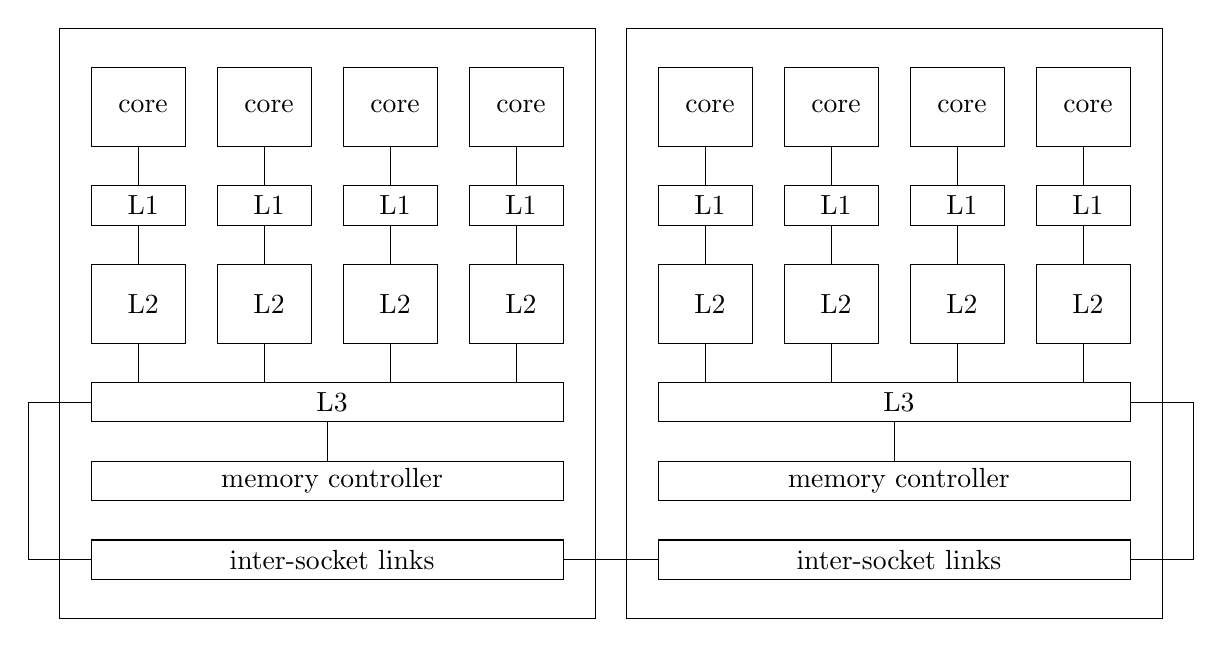
\begin{tikzpicture}[x=0.4cm, y=0.5cm]
                    \draw
                    (16, -13.5) -- (19, -13.5)
                    (1, -9.5) -- (-1, -9.5) -- (-1, -13.5) -- (1, -13.5)
                    (34, -9.5) -- (36, -9.5) -- (36, -13.5) -- (34, -13.5);
                    \foreach \i in {0, 18} {
                        \begin{scope}[shift={(\i, 0)}]
                            \draw
                            (0, 0) -- (17, 0) -- (17, -15) -- (0, -15) -- cycle
                            (8.5, -10) -- (8.5, -11);
                            \foreach \x in {1, 5, 9, 13} {
                                \begin{scope}[shift={(\x, -1)}]
                                    \node at (1.5, -1) {~core~};
                                    \node at (1.5, -3.5) {~L1~};
                                    \node at (1.5, -6) {~L2~};
                                    \draw
                                    (1.5, -2) -- (1.5, -3)
                                    (1.5, -4) -- (1.5, -5)
                                    (1.5, -7) -- (1.5, -8)
                                    (0, 0) -- (3, 0) -- (3, -2) -- (0, -2) -- cycle
                                    (0, -3) -- (3, -3) -- (3, -4) -- (0, -4) -- cycle
                                    (0, -5) -- (3, -5) -- (3, -7) -- (0, -7) -- cycle;
                                \end{scope}
                            };
                            \node at (8.5, -9.5) {~L3~};
                            \node at (8.5, -11.5) {~memory controller~};
                            \node at (8.5, -13.5) {~inter-socket links~};
                            \foreach \y in {-9, -11, -13} {
                                \begin{scope}[shift={(1, \y)}]
                                    \draw (0, 0) -- (15, 0) -- (15, -1) -- (0, -1) -- cycle;
                                \end{scope}
                            }
                        \end{scope}
                    }
                \end{tikzpicture}
            \end{center}
            With OLAP, as the number of threads increases, the throughput increases until a certain point where it begins to plateau.
            However, with OLTP, it initially goes up but then goes back down and plateaus at a lower level.
            This is due to the access latency and locking of shared data structures.
            On the other hand, the bottleneck with OLAP is due to the memory bandwidth.
            \medskip

            In practice, accessing the core to L1 only costs around 4 cycles and can be considered to be local.
            However, any of the lower layers can lead to stalls, which costs power and resources.
            Even in cloud workloads, over 50\% of the time (in most cases) goes to stalls, leading to approximately one instruction per cycle.
            In database workloads, for the \textit{Shore-MT} example, the stall cycles are dominated by L1I and L3D.
            For data intensive applications, between 50\% to 80\% of the cycles are stalls; due to instruction fetch and long-latency data misses (unavoidable; if we load unseen data, we are going to have a cache miss).
            To optimise this, we need to look at instruction cache locality as well as cache line utilisation for data.
            \medskip

            Some approaches for minimising memory stalls are as follows;
            \begin{itemize}
                \itemsep0em
                \item \textbf{prefetching}
                    \smallskip

                    Simple prefetching approaches include next line, where if we miss $A$, we fetch $A + 1$, or stream, where if we miss $A, A + 1$, then we fetch $A + 2, A + 3$.
                    This favours sequential access as well as spatial locality, however doesn't help with branches / function calls (where we need branch prediction), or pointer chasing (which can be done with the stride approach, where if we miss $A, A + 20$, we fetch $A + 40, A + 60$, in the case where we have a predictable structure).
                    The former is a case for instructions whereas the latter is a case for data.
                    These strategies are preferred on hardware as they are simple.
                    The penalty for a miss is a few cycles; if we exceed this to prefetch, we lose the benefit.
                    \medskip

                    Temporal streaming is based on the fact that programs tend to follow the same overall flow (in the way data and instructions are accessed) repeatedly.
                    The idea is to exploit recurring control flow; this is more accurate, however requires a higher space cost.
                    \medskip

                    An example of software-guided prefetching is when we visit a node, we may want to prefetch the children nodes.
                \item \textbf{being cache conscious}
                    \smallskip

                    An example of code optimisation is to simplify the code; in-memory databases have a smaller instruction footprint.
                    If the code is written to minimise jumps, it can better exploit the next line prefetcher.
                    The code can also be profiled for static optimisations, or just-in-time for dynamic.
                    Queries can also be compiled directly into machine code (rather than being interpreted on-the-fly).
                    \medskip

                    Data layouts can also be cache conscious.
                    Assume we have two 16-byte columns and a cache line of 64 bytes.
                    If our queries are ~SELECT *~, then a row store (good for OLTP) is beneficial, otherwise if our queries are in the form of ~SELECT <col>~, then a column store (good for OLAP) is beneficial.
                    The goal is to maximise the utilisation of the cache line as well as exploit the next line prefetcher.
                    \medskip

                    In the example of an index tree, if we are likely to perform a lookup-heavy workload, it should be stored in the visitation order of DFS, whereas if we have a scan-heavy workload (where we look at each level in order), it should be stored in memory in the BFS order.
                    The goal remains the same.
                    \medskip

                    The volcano iterator model passes a single tuple between operators.
                    A trivial improvement is to perform vectorised instructions which passes multiple tuples at a time between operators.
                    This provides good data and instruction cache locality, as well as allows for exploiting SIMD.
                \item \textbf{exploiting common instructions}
                    \smallskip

                    On executing the \textit{TPC-C} benchmark on \textit{Shore-MT}, the amount of data that is hot (reused often) is quite low.
                    However, the instruction reuse for certain workloads is quite high.
                    Consider a thread ~T1~ that has the instructions ~A,B,C,D~ and another thread ~T2~ that has the instructions ~A,B,C~, and 4 total cores.
                    In the first cycle, ~T1~ executes on core 1, leaving ~A~ in the cache.
                    In the next cycle ~T2~ executes on core 1, which already has ~A~ cached, and ~T1~ executes on core 2, leaving ~B~ in the cache.
                    Then ~T2~ executes on core 2, and ~T1~ executes on core 3, and so on.
                    The thread is executed on the core where the instruction is cached (if possible).
                    This approach is called SLICC.
            \end{itemize}
            In general, the problem with the L1I misses is due to capacity and can be solved by minimising the footprint as well as maximising reuse to create the illusion of a larger cache.
            LLC (L3) data misses can't be avoided, but we can maximise cache line utilisation with better algorithms and data layout.
            \medskip

            If multiple cores are accessing (modifying) the same data, locks need to be used to ensure safety.
            The data access pattern across threads is highly unpredictable.
            For each transaction, latching and locking accounts for a high number of critical sections.
            There are different types of critical sections (goal is to go from unbounded to fixed or cooperative);
            \begin{itemize}
                \itemsep0em
                \item \textbf{unbounded} \hfill all threads have access to centralised synchronisation point
                    \subitem many threads could want access at the same time; can be a major scalability bottleneck
                \item \textbf{fixed} \hfill fixed number of threads entering no matter how many threads in the system
                    \subitem not a bottleneck
                \item \textbf{cooperative} \hfill threads can combine requests as they're entering
            \end{itemize}
            To scale up OLTP, we need to consider the following;
            \begin{itemize}
                \itemsep0em
                \item \textbf{unscalable components}
                    \smallskip

                    Hot shared locks cause contention.
                    Consider multiple threads which all acquire different cold locks, but the same hot locks.
                    This leads to the same locks being released and requested repeatedly.
                    A solution is to perform speculative lock inheritance.
                    In this process, the first transaction commits \textbf{without releasing} hot locks and instead passes them to the next transaction which can either release them or use them, and so on.
                    This reduces lock contention.
                    \medskip

                    We want to move from centralised locking to thread-local locking, allowing each thread to use the locks as it pleases.
                    Predictable data access can be achieved by having a thread-to-data pattern; where each thread accesses the same subset of data.
                    This is beneficial as locks don't need to be passed between threads, since the data is on the same thread.
                    The same concept is used in in-memory databases.
                    \medskip

                    To reduce latching, we can use physiological partitioning (PLP).
                    An example of this is a multi-rooted B-tree.
                    Consider two workers, each working on half of the tree.
                    If we have something that access the first partition, the work is passed to the first worker, and similarly for the second partition.
                    \medskip

                    In a serial log performing WAL (write-ahead logging), locks are used to ensure that the threads write serially.
                    A number of methods can be used;
                    \begin{itemize}
                        \itemsep0em
                        \item \textbf{early lock release}
                        \item \textbf{flush pipelining} \hfill log writer on each thread and flush to the writer
                        \item \textbf{consolidation array} \hfill minimises log contention
                    \end{itemize}
                \item \textbf{synchronisation}
                \item \textbf{non-uniform communication}
                    \smallskip

                    Recall the diagram for the multiple sockets.
                    Accessing the L1 cache costs less than 10 cycles, accessing the L3 cache takes around 50 cycles, and accessing between sockets costs around 500 cycles.
                    As this is expensive, each socket should be considered an `island'.
                    OLTP on islands are as follows (similar ideas are in cluster computing);
                    \begin{itemize}
                        \itemsep0em
                        \item \textbf{shared-everything} \hfill everything is shared between sockets and cores
                            \subitem sub-optimal due to the cost of accessing between sockets.
                        \item \textbf{island shared-nothing} \hfill cores on the same socket share
                            \subitem good middle ground, avoids expensive inter-socket communication
                        \item \textbf{shared-nothing} \hfill nothing is shared, even between cores
                            \subitem fast, however it's sensitive to the workload
                    \end{itemize}
                    The challenge lies in configuring the workload for the hardware, as repartitioning is expensive.
                    Adaptive Transaction Processing use the system state to determine how we want to run tasks.
                    It makes shared-everything system scalable on islands and adaptive to any changes to the hardware / workload.
                    PLP is used between islands, and uses different threads to access data on different subsets of the data, located on different islands.
            \end{itemize}
            Scaling up OLTP involves identifying bottlenecks in existing systems (and eliminating them).
            We also cannot assume uniformity in communication (different orders of magnitude of time to access different data).
            The correct synchronisation mechanisms should also be chosen.
        \subsection*{October 28 - Live Lecture}
            Predictions cannot take longer than a stall, so very simplistic models need to be used.
            \medskip

            We need to ensure we isolated updates (either on the level of a table or row).
            Some care might need to be taken for reads as well (to ensure data isn't being read during an update).
            \medskip

            In speculative lock inheritance, we pass hot locks between transactions, after committing.
            \medskip

            Shared-everything, in distributed computing, works well when there is low latency between islands.
            However in the case of sockets, there is (relatively) high overhead.
            Shared-nothing requires the work to be partitioned where everything is local.
            \medskip

            In serial logging, the transaction that will be executed is written into the serial log (persistent).
            However, not every transaction can write at the same time, hence access to it needs to be serialised.
            The idea for flush pipelining is to start writing, but start working on other tasks when waiting; not improving latency but improving throughput.
        \subsection*{6.1 - Cold Storage}
            Data can be classified by how frequently it's accessed (as well as size).
            The amount of data is growing rapidly, however the majority of it is infrequently accessed (cold) - compared to frequently accessed data (hot).
            The goal is to find a good tradeoff between price and performance; it doesn't make sense to store all cold data in SSD.
            Archival data is typically written once and quite likely to never be read, and is stored on tape (we don't care about latency).
            Cold storage devices (CSD) fit between the hot / warm tiers and the archive tier.
            The cold tier has low hardware costs and a lower latency than tape.
            \medskip

            A key idea is adequate provisioning.
            We want to provide just enough cold storage resources just for the cold data workload.
            Disks could be archival and SMR, rather than standard commodity drives.
            We also want to limit power, cooling, and bandwidth - there's no need to provision for peak power and have all the disks spinning all the time; just enough disks spun up to saturate bandwidth.
            The advantage of removing unnecessary resources include low hardware costs and operating costs, as well as a high density of storage.
            \medskip

            An example for this is \textit{Microsoft Pelican}, where only $\frac{1}{K}$ of the disks are active ($\approx 8\%$) - one disk group spun up.
            Spinning up a new group of disks (disk switch latency) is between 10 and 30 seconds.
            The workload that CSDs fall under is known as WORO; write once read occasionally.
            \medskip

            The \textit{Pelican} rack has a very high storage density (52U with 1152 archival 3.5" SATA disks, approximately 5 PB of storage); achieved by removing unnecessary infrastructure / hardware - for example fixed cooling channels.
            It's designed to store blobs which are partitioned into multiple chunks.
            Management is made simpler by grouping the disks into domains (limits on the following);
            \begin{itemize}
                \itemsep0em
                \item cooling \hfill only 2 disks can be active at a time in a group
                \item power \hfill only 1 disk active at a time in a group
                \item bandwidth
            \end{itemize}
            Disks use resources from a set of resource domains (which are provisioned to supply resources to a subset of disks).
            Disks are either domain-conflicting (same resource domain) or domain-disjoint (share no common resource domains).
            The slides contain a representation of this.
            \medskip

            This is generally more of an object store than a file system.
            Each blob is stored over a set of disks (split into a sequence of 128kB fragments - for each $k$ fragment, additional $r$ fragments are generated for error correction, the $k+r$ fragments form a stripe; if $k = 15$ then $r = 3$).
            \textit{Pelican} statically partitions disks into groups (disks can be concurrently active); conflicts are concentrated over a few sets of disks.
            The lecture then goes over the placement of data.
            Two groups can be fully colliding / conflicting, but if none of the disks in the same group is colliding then it can all be accessed at the same time.
            \medskip

            Traditional schedulers reorder IOs to minimise seek latency, whereas \textit{Pelican} reorders the requests in the queue (read / write) to minimise the impact of spin up latency.
            \textit{Pelican} also has a reordering operation (similar to disk defragmentation); the scheduler is more likely to write to an active (spinning) disk than to spin up a different disk.
            \medskip

            The implementation needs to ensure that disks are powered up in standby, to ensure it doesn't spin up without \textit{Pelican} managing the constraints.
            Group abstraction is exploited to parallelise the boot process - the most important aspect of the groups is to simplify scheduling (if we don't have groups, we need to consider which other disks it conflicts with; there are 3 domains and 1152 disks to consider).
            \medskip

            The next section discusses \textit{Pelican} compared against a system that has full provisioning for power and cooling; same organisation (physical internal disk topology), but the disks are never spun down (obviously better for latency).
            As expected, the throughput for FP goes up as the number of requests go up (until it hits the bandwidth limit), whereas \textit{Pelican} does something similar however hits a limit earlier due to the group switching (and one group not entirely saturating the bandwidth).
            The time it takes to read the first byte for \textit{Pelican} starts around the 14.2 second point (the average time it takes to activate a group), but as requests goes up it becomes the same value as the FP.
            However, for power consumption with all disks spun down (just powering system), the draw is at 1.8kW, whereas for the \textit{Pelican} peak, it's at 3.7kW, and for all disks active, it's at 10.8kW.
            \medskip

            The benefits of this are reduced cost and power consumption (right-provisioned), has accuracy from error codes, and abstraction simplifies IO scheduling.
            On the other hand, it's not flexible to changes and is sensitive to hardware changes.
            \subsubsection*{Data Processing}
                In the traditional setting, we typically had a database accessing a disk, with uniform access, a controlled layout, and static (pull-based) execution, all done via blocks.
                On the other hand, we're likely to have multiple databases reading objects over the network for the cold storage tier.
                There is no longer uniform access or controlled layout, and pull-based execution will lead to group switches.
                \medskip

                We cannot just simply replace HDD with CSD in the background, as it will have an impact on the software.
                Therefore we require hardware-software co-design; access needs to be hardware-driven to minimise group switches.
                Execution engine has to process the data from storage in an out-of-order / unpredictable manner.
                Data round-trips should also be reduced with smart caching.
                \medskip

                Common batch processes on CSD include;
                \begin{itemize}
                    \itemsep0em
                    \item massive-scale group-by / join
                    \item duplicate detection
                    \item data localisation
                    \item in-place map-reduce
                \end{itemize}
                We typically don't do operations on cold data, but when we do it should still be done efficiently.
                Data needs to be partitioned into $K$ groups to be distributed between $K$ disk groups.
                Data from each disk group is read into memory (buffer), partitioned, and then flushed to the different disk groups - allowing the a CSD group to have partitions $1$ to $m$ and then the next group having partitions $m + 1$ to $n$, and so on.
                \medskip

                However, when the buffer is full, we need to flush it.
                The naive approach is to flush a partition once it's full, and then fill up just that partition.
                However, this leads to many switches.
                The Buff-Pack approach tries to avoid switching by flushing to the current disk group if possible, otherwise it switches to the disk group with the largest buffer.
                The intuition for the Off-Pack approach is that we flush the entire buffer (into the current disk group) even if it's in the wrong group.
                After the flush, all of the offload buffer is moved.
                \medskip

                The estimated total time is as follows, note that the switching time dominates this;
                $$T_\text{total} = T_\text{switch} + T_\text{seek} + T_\text{read} + T_\text{write}$$
                In general, Off-Pack performs better as it has fewer switches and more read / writes.
                It's better for a smaller buffer, high number of disk groups, and high throughput.
                For a low number of disk groups and smaller switch latency, Buff-Pack can outperform Off-Pack.
                Off-Pack works well with smaller buffer sizes, however as the size gets larger, Buff-Pack performs better.
        \subsection*{6.2 - DNA Storage}
            An issue with tape storage is that 60\% of archival data is stored for longer than 20 years, however tape has a lifetime of 10-20 years.
            This means that the data needs to be migrated every couple of years.
            A similar issue is present with microfilm, called vinegar syndrome, causing the film to disintegrate.
            \medskip

            DNA has been synthesised for medical purposes.
            It offers a higher volumetric information density (gigabits per cubic millimetre) than other mediums, with a potential $10^7$ improvement over existing storage media.
            Additionally, it's also very durable.
            The demand for silicon is also starting to exceed the global supply.
            Finally, biological operations on DNA are highly parallel (millions, if not billions of operations in parallel).
            \medskip

            DNA is a double, long chain of molecules called nucleotides (A, T, C, and G).
            The complementary nucleotides (A / T, and C / G) provide stability.
            \medskip

            To store information, the binary information is encoded into nucleotides, synthesised into DNA, sequenced back into the nucleotides, and then finally decoded back into binary.
            The goal is to minimise the number of nucleotides per bit, as it's still quite expensive.
            A simple encoding would be $~00~ \to ~A~, ~01~ \to ~T~, ~10~ \to ~C~, ~11~ \to ~G~$, which would theoretically have have half a nucleotide per bit.
            However, there are biological constraints; for example we can't have too many of the same nucleotide in a row as it leads to breakages.
            Additionally, synthesis and sequencing are error-prone.
            In reality, we have the following, with an \violet{identifier / offset}, \teal{error correction codes} to account for errors in the aforementioned steps, and the actual \blue{value};
            \begin{center}
                \violet{~AGG~}\teal{~CTCAGAT~}\blue{~AGATCTAATT~}
            \end{center}
            This leads to around 1 nucleotide per bit.
            There are also biological constraints on the length of the sequence, due to the technology to synthesise but also the likeliness of breakage in longer sequences.
            As such, data may need to be broken down into an array of sequences, and can be addressed by the identifier.
            \medskip

            If we have two structures which are perfectly complementary, they are highly likely to bind together.
            This has been historically used to solve combinatorial problems, and can also be used for database joins.
            The idea is to exploit chemical processes;
            \begin{itemize}
                \itemsep0em
                \item annealing of complementary nucleotides
                \item polymerase chain reaction (PCR) to replicate / amplify DNA sequences
                    \smallskip

                    Content retrieval through amplification.
                    We need to know the beginning of the sequence and the end of the sequence.
                    If we have a mix of sequences, we can apply PCR with the knowledge to create millions of copies, leading to it dominating the mix.
                \item loop-mediated isothermal amplification
                    \subitem content detection
            \end{itemize}
            A simple approach is to encode a binary dump of the database.
            This wastes space on the identifier ($\log_4(|\text{segments}|)$), doesn't support point queries, and near-molecule data processing can't be performed.
            Reassembling this would require clustering and reassembly, which is a necessary but time-consuming step before decoding.
            \medskip

            A structured data layout approach is to use NSM on DNA, with one row per oligo (short single strands of synthetic DNA).
            The unique primary key is used to avoid extra indexing.
            DSM on DNA is a columnset partitioning for large rows, which keeps the primary key and a \textbf{single} field.
            With structure-preserving encoding, the DNA read restoration can be mapped to a data cleaning operation.
            \medskip

            To perform point queries, we can use PCR with the table and column ID as the start sequence, and the value as the end sequence.
            $$\underbrace{~AGG~}_\text{start}\underbrace{~CTCAGAT~}_\text{PK}\underbrace{~AGATCTA~}_\text{ECC}\underbrace{~ATT~}_\text{end}$$
            \subsubsection*{Join}
                The goal is to use the complementarity (matching base pairs) to anneal complementary single stranded oligos.
                Matching records / attributes have complementary encodings of the values.
                \medskip

                Each attribute is encoded as before, but with an additional reversed oligo with the value complemented (~TAAAGATCTACTCAGATAGG~).
                If this reversed oligo matches a non-reversed oligo, the values will be perfectly complementary (exactly anneal).
                See the example below - note the three nucleotides in parentheses on either line are the table and column IDs, and the square brackets are the complementary values.
                \begin{lstlisting}
                    (AGG)CTCAGATAGATCTA[ATT]
                                       [TAA]ATCGAGGGATTACA(TTT)
                \end{lstlisting}
                However, this could lead to wrongly annealed pairs.
                PCR is then used to obtain only the chains which have annealed and are the IDs we are looking for.
                If they anneal, they are twice the weight of a single sequence.
            \subsubsection*{OligoArchive}
                The idea is to implement all the layers of the storage stack alongside automation on all layers;
                \begin{itemize}
                    \itemsep0em
                    \item \textbf{application layer} \hfill encoding structured (database) and unstructured (imaging) data
                    \item \textbf{OS layer} \hfill file system abstraction
                    \item \textbf{controller layer} \hfill data processing capabilities
                    \item \textbf{media layer} \hfill synthesis and sequencing
                \end{itemize}
                Nanopore sequencing pulls DNA through a membrane which unzips the helix into two strands.
                Each base blocks the flow to a different degree, altering the current which can then be used to identify them electronically.
                \medskip

                The current roadblock is the synthesis cost.
                For medical purposes, the synthesis has to be precise, but for storage purposes there is some tolerance for errors.
                Other approaches include longer sequences, longer alphabets (more nucleotides), and synthetic molecules.
                \medskip

                Current research is looking at encoding, synthesis costs, synthetic molecules, automation, and packaging / storage (wrapping long sequences around synthetic histones).
        \subsection*{November 1 - Live Lecture}
            Synthesis cost can be reduced by pre-fabricating sequences and then replicating with PCR.
        \subsection*{November 4 - Lecture 1}
            As \textit{Google} search grew, the number of search queries exploded.
            Back in 1999, it took a month to retrieve 50 million pages (limited by internet speeds and web server speeds), but in 2012, it took less than a minute.
            These advances were enabled with using lots of machines to scale services; a single typical query may access thousands of machines in just a few hundred milliseconds.
            \medskip

            Performance correlates with user experience; we expect them to be interactive / instantaneous.
            Any latency has direct business impact, with services losing money if the latency of the service increases - for example, \textit{Amazon} saw direct drops in sales when the service is slow.
            \medskip

            Another consideration is scalability; as services grow the infrastructure needs to scale effectively.
            We ideally want linear scalability, the workload is directly proportional to the resources (such as number of machines).
            However, this isn't easily achievable, due to overheads from synchronisation between machines, imbalanced loads across the infrastructure, and similar.
            Techniques that are applied to make services scalable.
            \medskip

            A major barrier for entry to using a supercomputer / mainframe / HPC was the cost - being too high for a startup.
            This also has issues with scaling; once the box is filled with the maximum number of CPUs, another machine would have to be purchased, which may then be too much performance for the work - the companies ideally wanted incremental scaling, without large upfront costs.
            A significant amount of the cost from these machines comes from the reliability and the redundancy built in.
            If some of the mechanisms for reliability can be pushed into the software, less reliable hardware can be used.
            \medskip

            Most scalable services moved towards distributed computing, with a client / server model.
            The computing infrastructure instead uses commodity hardware, which could be easily purchased cheaply in bulk, giving a good price versus performance tradeoff.
            However, considerations had to be made regarding the reliability (previously, supercomputers would hide the failures from software).
            Additionally, servers in a data centre have limited bandwidth and higher latency (compared to tightly interconnected CPUs in a supercomputer); leading to expensive communication.
            \medskip

            Distributed systems have the following properties;
            \begin{itemize}
                \itemsep0em
                \item \textbf{scalability}
                    \smallskip

                    Resources should be aggregated, including compute resources, storage, memory, and bandwidth (e.g. with CDNs).
                \item \textbf{location transparency}
                    \smallskip

                    The client doesn't know what data centre the request is being handled by, let alone the individual server.
                    This gives significant flexibility by hiding the implementation of the infrastructure from clients.
                \item \textbf{high availability}
                    \smallskip

                    We want systems that are always up and available.
                    There's significant redundancy in the hardware design (companies don't want the entire data centre to fail as a whole), despite individual servers failing.
                    Hardware and software failures should be masked.
                \item \textbf{composable services}
                    \smallskip

                    Composable services allow companies to easily deploy and launch new services and applications from basic building blocks.
            \end{itemize}
            In a search request, the request is routed to a server, possibly based on DNS.
            The web server then communicates with other servers, including multiple index servers and document servers, as well as other services, such as advertising and spell checking.
            The computation required for a search query is distributed to other servers (working in parallel), by partitioning the work with subqueries.
            The web index is partitioned into shards in index servers, and pages (documents) are also partitioned in a similar way.
            The latency to handle any particular query is low as the computation required to look up anything in the search index is low (since it's all done in parallel).
            A similar technique is used by most web services.
            \begin{enumerate}[1.]
                \itemsep0em
                \item load-balancer routes request to lightly loaded GWS (\textit{Google Web Server}) - the goal is to have all servers with roughly the same load (a single overloaded server would cause all requests to that server to have higher latency).
                \item GWS routes search to one index server for each shard - a search keyword is looked up in all indices
                \item IDs of the matching pages being returned from the index servers; these results are aggregated (sorted by relevance)
                \item GWS sends IDs to document servers to obtain metadata
                \item results are aggregated, with advertisements etc., producing a search result page
            \end{enumerate}
            A similar structure is followed for generating \textit{Amazon}'s front page, as it's customised to the customer.
            \medskip

            Data centres contain the computers used to run these services, and are typically commodity hardware (with non-commodity networking).
            The assumption is that we scale out (install more commodity servers) rather than scaling up.
            Software needs to be designed to tolerate failure.
            Due to the scale of a data centre, everything follows economies of scale, for electricity, hardware, network, and operations.
            The larger the data centre, more is invested in automation (thus reducing the amount of manual administration).
            \medskip

            With the scale out model, load spikes can be handled on demand.
            This is especially important for services where popularity can suddenly spike (such as viral videos).
            An initially unpopular server would have a smaller allocation of servers, but as load and popularity grows, a larger allocation would be provided.
            This creates an illusion of infinite resources.
            Large scale data centres are typically located close to cheap electricity, such as near hydroelectric dams.
            \medskip

            There's some separation for the requirements on the scale of a distributed system;
            \begin{itemize}
                \itemsep0em
                \item \textbf{online systems} (latency matters, below 100ms), e.g. OLTP, interactive, web content
                \item \textbf{batch processing system} (above 1 hour) - don't care about getting a result back instantly, includes offline data processing, data analytics and warehousing, focuses on processing data effectively
                \item \textbf{nearline systems} (latency can be higher than online systems, below seconds or minutes), dynamic content to users where freshness matters, such as recommendations, advertisements, and dashboards (monitoring, debugging, etc)
            \end{itemize}
            A single page may use multiple of these; for example a feed may need to be online, but advertisements on the page don't be.
            \medskip

            Challenges include scalability and fault tolerance, but also require consistency.
            When a system has data replicated in different locations, independent updates may cause different copies to become inconsistent.
            Some of these challenges are solved with abstraction; applications are run on top of the highest layer.
            Each layer is scalable, network-aware, and fault-tolerant, for example, \textit{BigTable} sits on top of the distributed file system, which handles replicating files across servers.
            A \textit{MapReduce} computation can then sit on top of \textit{BigTable}.
            As long as each layer is scalable, the entire stack is also scalable, as well as any applications on top of this stack; the same is true for fault-tolerance.
            \medskip

            The design principles for scalable systems include (not exhaustive);
            \begin{itemize}
                \itemsep0em
                \item \textbf{stateless services}
                    \smallskip

                    Dealing with state or data is challenging.
                    If data isn't replicated, we need to ensure it's not lost, and if it is replicated, then we need to worry about consistency.
                    HTTP is a stateless protocol; the request is entirely self-contained (has all the information the web server needs to get a response); any subsequent request doesn't need to remember information about a previous request.
                    This helps the web scale well, as each server can easily handle concurrent accesses.
                    Any state in modern websites is pushed into the database tier (not in the protocol, or the presentation tier).
                    Between these two tiers, there's the logic / application tier.
                    As this is all stateless, we can easily add more web servers to help load balancing.
                \item \textbf{caching}
                    \smallskip

                    Latency is important in many of the systems we are building.
                    Caching data closer to client such that it can be retrieved quickly helps with latency.
                \item \textbf{partition / aggregation pattern}
                    \smallskip

                    Parts of a query can be completed on partitions in parallel and then aggregated to get the final result.
                \item \textbf{weaker consistency}
                    \smallskip

                    Consider data that is copied to two different data centres.
                    Assume there are two clients who are accessing / modifying the data concurrently, which could lead to inconsistency.
                    An idea is to weaken the consistency guarantees, which can help with the scalability of the services by reducing the communication between servers.
                    \medskip

                    Many applications may use a mix of strongly consistent operations (often adds additional latency) and inconsistent operations.
                \item \textbf{efficient failure recovery}
                    \smallskip

                    Making everything redundant is too expensive.
                    The two main techniques are replication (another copy exists if one is lost or recomputation (redo a computation if the result is lost).
                    The cost of failure recovery needs to be low, as failure is the norm.
            \end{itemize}
        \subsection*{November 8 - Lecture 2}
            The cloud is really just the data centre hardware and associated software stack.
            Virtualisation hides the details of these resources from applications and exposes them in a certain way.
            The cloud is a pool of easily usable virtualised compute resources, development platforms, services and applications.
            Cloud computing is the delivery of computing as a service, with multi-tenancy (provide resources to multiple tenants but isolate them from each other).
            The cost of this is based on the resources consumed.
            \medskip

            The main advantages of cloud computing to the user is that they don't need to have physical hardware and can get resources on demand (for example, incremental scaling with horizontally scaling services).
            The cloud provider also looks after the hardware and parts of the software stack, as well as the security.
            \medskip

            Issues include the dependency on a network connection, which can be an issue for availability.
            There are also security and privacy issues, with trusting the provider with data and computation, as well as complicating legal issues.
            Another concern is vendor lock-in (and cost of migration), as a provider wants a user to stay (possibly making it expensive to move if infrastructure is built on certain services).
            This is less of a concern with standardised microservices.
            \medskip

            The typical distinction is as follows;
            \begin{itemize}
                \itemsep0em
                \item \textbf{public cloud}
                    \smallskip

                    The typical providers we are familiar with, simply requiring payment to use.
                \item \textbf{private cloud}
                    \smallskip

                    Cloud environment used by a single organisation.
                    The use of virtualisation and abstraction is similar to that of a public cloud, but is run by a single organisation for the use of tenants within the organisation.
                \item \textbf{hybrid cloud}
                    \smallskip

                    Combination of both public and private clouds.
                    For example; an organisation with a private cloud but some workloads are run on the public cloud (for non-sensitive data).
            \end{itemize}
            The different cloud services models (abstractions provided) are as follows (in order of most control to the user to least);
            \begin{itemize}
                \itemsep0em
                \item \textbf{Infrastructure-as-a-Service (IaaS)}
                    \smallskip

                    Exposing hardware in a virtualised way.
                    For example, exposing a VM allowing the user to install their own OS and software.
                    \medskip

                    Raw resources are provided; for example storage, processing, memory, and network bandwidth.
                    The virtualisation layer is a privileged software layer that exposes the hardware resources in a safe way across servers.
                    VMs are isolated from each other and have their own regular software stack.
                \item \textbf{Platform-as-a-Service (PaaS)}
                    \smallskip

                    Slightly higher level abstraction, for example containers (microservice based applications).
                    Abstracts away from the raw hardware.
                    No overhead of having to manage an OS as a user would do in a VM.
                    \medskip

                    More of the stack is managed by the cloud provider, including the O/S, middleware, and runtime, reducing the tenant's management overhead.
                    The user manages the data and the application itself.
                \item \textbf{Function-as-a-Service (FaaS)}
                    \smallskip

                    This considers applications as individual functions that need to be invoked.
                    The provider provides an API to accept a function and invoke the function.
                    Elasticity is easier to achieve (from the user's perspective), as the cloud provider now manages the number of instances.
                    \medskip

                    This is also referred to as serverless computing (the concept of the server is hidden from the tenant, hiding away decisions such as the number of CPU cores or amount of memory).
                    The application the user wants to run is split at a finer granularity.
                    However, the functions must be short.
                \item \textbf{Software-as-a-Service (SaaS)}
                    \smallskip

                    Particular cloud hosted applications, accessed over the Internet.
                    For example, \textit{Office 365}, or \textit{Dropbox}.
                    The underlying software is handled by the cloud provider.
                    \medskip

                    The cloud tenant has much less control over the customisation, as they are only consuming a service.
            \end{itemize}
            \subsubsection*{Data Centres}
                Efficient management of a data centre allows the cloud provider to pass cost savings to the customer.
                IaaS is generally interchangeable between providers, hence users typically go to the cheapest provider.
                \textit{Microsoft} attempted submerging a data centre under the sea, for the purpose of cooling (a large cost for providers).
                \medskip

                Data centres need to optimise for a number of things;
                \begin{itemize}
                    \itemsep0em
                    \item reliability \hfill mirrored data centres
                    \item geographic diversity, locations of data centres
                    \item time to recover in the case of an outage
                    \item future expansion
                    \item power requirements \hfill ideally cheap electricity
                    \item connectivity \hfill multiple independent connections to the Internet
                    \item physical security
                \end{itemize}
                The standards for infrastructure as follows;
                \begin{center}
                    \begin{tabular}{llllll}
                        \textbf{tier} & \textbf{generators} & \textbf{UPSs} & \textbf{power feeds} & \textbf{HVAC} & \textbf{availability} \\
                        \hline
                        $1$ & none & $N$ & single & $N$ & $99.671\%$ \\
                        $2$ & $N$ & $N + 1$ & single & $N + 1$ & $99.741\%$ \\
                        $3$ & $N + 1$ & $N + 1$ & dual, switchable & $N + 1$ & $99.982\%$ \\
                        $4$ & $2N$ & $2N$ & dual, simultaneous & $2N$ & $99.995\%$
                    \end{tabular}
                \end{center}
                All critical systems need redundancy (for example, a power outage in a region can be overcome with a diesel generator).
                The power distribution may fail and a data centre might have redundant power feeds.
                Redundancy is required in cooling as well.
                \medskip

                See the slides for the components of a data centre.
                Data centres have a battery system for redundancy to bridge the gap between an outage and the diesel generators starting up.
                \medskip

                A rack holds between 40 to 80 servers.
                Each rack typically has a network switch associated with it, which are then interconnected to allow for full connectivity between all the servers in the data centre.
                \medskip

                Another model for data centres is having them in shipping containers.
                These containers can be kept on hand for replacement and there is already an existing network that can transport shipping containers efficiently.
                Servers can also be left to fail within the containers (masked by software), and once this failure rate exceeds a certain threshold, the entire container can be ordered and replaced.
                \medskip

                Edge computing avoids having a single large compute data centre, but rather smaller data centres located closer to users.
                This can possibly cause issues with economies of scale, similar to the shipping containers.
            \subsubsection*{Cost and Utilisation}
                The TCO (total cost of ownership) of running a data centre is the sum of CapEx (capital expense; upfront investments) and OpEx (operation expenses; monthly costs including electricity and maintenance).
                Cloud computing removes the CapEx part, but the cost of hardware shifts towards OpEx.
                \medskip

                A third of the monthly operating cost of a DC comes from power; both to operate the servers and to cool them.
                The PUE (power usage effectiveness) is the ratio of the total energy used by a DC to the actual useful work (energy delivered to the computing equipment).
                Cooling is one area where operators can reduce costs.
                For example, running a DC at a higher temperature can lead to higher failure rates of components, but can save cooling costs.
                Another option is going to a cooler climate or locations with cheaper energy.
                \medskip

                A typical layout of a DC has hot and cold aisles; the former used to transport hot air out of the data centre, and the latter to blow cool air into the servers.
                Small improvements in efficiency in cooling can achieve savings in lower energy costs and lower failure rates.
                \medskip

                Ideally, servers in a DC are energy proportional, where the power usage is directly proportional to the utilisation (amount of work).
                For example, if the server is doing no work, there should be no energy usage.
                Modern servers are better at being energy proportional, partially due to the technologies in mobile devices.
                \medskip

                Very few servers in a DC are fully utilised, with a peak around 30\% usage.
                When there is redundancy, a standby server will be idle, which reduces average utilisation.
                When the utilisation of a system is high, there are more queuing delays, leading to higher response times (and poor tail latency) - therefore when optimising for lower tail latencies, we want to be in an area of lower utilisation (less queuing).
                Tail latency refers to the $99^\text{th}$ percentile (or higher) of latency.
                \medskip

                Virtualisation allows for consolidation of workloads, therefore increasing the utilisation certain machines (concentrating the usage on certain servers).
                A software defined data centre has the goal of doing more in software than hardware.
                When management functions are implemented in software, there is more control over the policy and how it works.
                Hardware load balancers are difficult to configure as the load balancing was implemented in hardware, requiring changes to the firmware to modify behaviour, whereas software based balancers allow for more complex policies.
                \medskip

                VM (live) migration is one of the advantages of using VMs.
                This is entirely transparent to the application.
                A VM can be migrated by starting to copy memory into another server, and once it has copied most of its memory and is synchronised with the other server, it can stop and copy over the remainder of the memory.
                \medskip

                Cloud providers avoid oversubscribing memory as the effect of thrashing is very noticeable.
                On the other hand, CPU degradation is less noticeable.
                \medskip

                Networking is another challenging area of data centres.
                In the past, a few companies had a monopoly on networking equipment, including \textit{Cisco} and \textit{Juniper}.
                Software defined networking has switches as usual, but all of the routing decisions are controlled by the data centre operators.
                It doesn't make sense to run regular Internet routing protocols when running a DC.
            \subsubsection*{Rack Scale Computing}
                Instead of considering a basic compute unit as a single server, rack scale computing thinks of the basic unit of computing as the entire rack.
                A rack-scale computer has standard compute units as well as accelerators (such as GPUs), as well as storage units (for different `temperatures' of storage).
                This helps to achieve higher densities.
                \medskip

                The current view of servers is that they include the resources; the server interconnects the CPU, memory, storage, etc.
                In a rack scale design, the server still has the same role, but at a rack scale.
                However, in a resource-centric design, the data centre network has the resources directly connected to it (disaggregated resources).
                This allows for exactly the required resources to be added.
                This is possible nowadays due to the ability to have lower latencies between resources due to newer technologies.
        \subsection*{BigTable}
            The idea of BigTable was to design a scalable distributed system that's reliable but also easy to reason about.
            Existing DB systems couldn't be used by Google not only due to the scale of the data, but also the requirement to provide low latency services for a variety of workloads.
            The amount of data that can be handled by the database system also needs to be able to scale incrementally.
            Another motivation for creating their own solution is licensing costs; parallel databases already existed but would be expensive.
            \medskip

            Some key novel ideas are;
            \begin{itemize}
                \itemsep0em
                \item
                    Users are allowed to select locality criteria (based on application needs, data will be accessed from similar locations in GFS).
                    When distributing data, it's important to consider what bits of data should be kept together.
                    Locality is important for a system like BigTable; if the data is distributed, data would have to be retrieved from many different machines (latency penalty).
                    See families in the next point.
                \item
                    BigTable introduced a semi-structured data model (between a fully structured relational model and a key-value store).
                    The design choice came from their use-case of web search.
                    It starts with a simple key-value model, but the key is made richer with column keys, and families (which influence locality, and can help a programmer categorise the data).
                    The key can be thought of as a compound key, consisting of a row key, a column key, and a timestamp.
                    This is still different from a relational database model (despite the compound keys having columns) as the format isn't enforced.
                    Another difference is that relational models tend to be unordered and don't have row keys (the key comes from a column).
                \item
                    Another aspect of the model is versioning (timestamps).
                    At the time, this was a new feature.
                    This feature made sense for the use cases as the links between web pages are quite dynamic (but the company may want to keep old versions).
                    This also helps to improve the speed as an update just involves adding a new version, without removing / replacing the old one.
                \item
                    Immutability (mostly), rows are copied on write, preventing race conditions.
                    An SSTable provides a persistent, ordered immutable map from keys to values (both are arbitrary byte strings) - once data is written, it can never be changed.
                    Deletion is done by adding a new record that marks something previously stored as deleted.
                    The table is ordered on the row keys (generally an expensive operation) - this gives the benefit of being able to do binary search on the data (avoid the cost of a full linear scan).
                    Immutability also helps to remove the need to synchronise access to SSTables; consistency is very easy when nothing can be updated.
                    \medskip

                    Consider SSTables as simply files on a distributed file system (GFS).
                    Replication is done at the level of the file system (therefore BigTable doesn't have to deal with it).
                    However, GFS doesn't know about locality, therefore it's important for data that we want to store together (locality) to be in the same SSTable (same machine).
                \item
                    Compactions essentially group together updates, in a cleanup operation.
                    This removes old data (either marked as deleted, or data that has been updated).
                    Without a compaction mechanism, data is never deleted (this is similar to a garbage collection process).
                \item {}
                    The memtable stores recently committed updates.
                    When a write / update occurs, the memtable is updated, and when it gets large, compaction occurs.
                    On a read, the updates from the memtable are used with the results in the table (the union of the memtable and the SSTable is taken).
                    The memtable can be thought of as an SSTable that's in memory, and is also sorted (can be done quite cheaply on an insert).
                    Write queries are therefore very cheap, but reads are a bit more expensive.
                    \medskip

                    A tradeoff is made here to give writes lower latency, as they are more important and bring data into the system.
            \end{itemize}
            BigTable is motivated by Google's scale (to support other applications than search), with no commercial system big enough.
            This uses the following building blocks (existing services within Google);
            \begin{itemize}
                \itemsep0em
                \item \textbf{Google File System}
                    \smallskip

                    This is a large-scale distributed file system that stores the actual data.
                    There is a master server responsible for metadata, such as where the files are stored, as well as chunk servers which store the actual data.
                \item Chubby Lock Service
            \end{itemize}
            There support for a query language, but an API is provided for lookup, insertion, and deletion.
            Indices don't exist in BigTable (no need, as it's already ordered).
            Transactions don't exist in BigTable either, but each read / write of data under a single row key is atomic (multiple updates can't be done atomically).
            Proper transactions (multi-row updates, for example) don't exist as they don't care about consistency and would add too much complexity.
            The main differences to traditional relational databases are;
            \begin{itemize}
                \itemsep0em
                \item no table-wide integrity constraints
                \item no multi-row transactions
                \item no aggregation over data; values are uninterpreted
                \item data is immutable (similar to versioning databases)
                \item functions, no SQL
                \item clients indicate what to cache in memory
                \item no index, data is stored lexicographically (locality is controlled by naming of rows and columns)
            \end{itemize}
            The SSTable is subdivided into 64KB blocks, which is the granularity at which I/O works on.
            An index is also present, which denotes which block a particular key resides in.
            A tablet is a collection of SSTables; and stores a consecutive range of rows keys from the overall data.
            The highest form of organisation is the table, which are then subdivided (sharded) into tablets (which contain SSTables).
            Tablets are the the unit of data that are actually being assigned to servers in a data centre; each tablet is assigned to a tablet server.
            The mapping of tablets to tablet servers is unique (each tablet is served by exactly one tablet server).
            \medskip

            We can't control what range of keys go to a specific SSTable.
            Every SSTable starts as a memtable (in memory), and once it gets large, it is then written out to disk.
            Therefore a a tablet may split an SSTable (an SSTable can be shared between two tablets) - this is fine as the tables are stored in GFS, as any tablet can access any SSTable, and a unique mapping is still maintained.
            Reads are expensive, as we know the set of SSTables that may contain the data, but we have to look at all the SSTables associated with the tablet as they may contain the latest version of the key.
            While tablets don't overlap, SSTables can overlap (compactions get rid of the overlap) as we just create tables based on writes (the range of keys in an SSTable can overlap, but the range of keys in tablets don't).
            \medskip

            There are three types of compactions (the cost of writing to disk is delayed to the compactions);
            \begin{itemize}
                \itemsep0em
                \item minor
                    \subitem converts a full memtable into an SSTable
                \item merging
                    \subitem take a bunch of SSTables under a tablet and combine them to reduce the number of SSTables, can remove data marked as deleted
                \item major
                    \subitem ensures there are no overlapping key ranges
            \end{itemize}
            A write operation first goes onto a log, which is an append-only log file on GFS (not sorted, can be efficiently appended with sequential I/O).
            This prevents data from being lost if there's a failure in a tablet server, as the memtable only lives on memory.
            The memtable can be reconstructed by replaying the log.
            The log can be truncated when the memtable is written to disk; the only data that needs to be on the log is data that is on the memtable.
            \medskip

            The performance will depend on how well the queries are balanced across the servers.
            The master needs to be fault tolerant; it knows the assignment of tablets to tablet servers.
            The metadata table is also stored in BigTable (bootstrapping); the root tablet contains information about where all the other metadata tablets are, which contains information about where all the user data tablets are stored.
            However, this can't be stored in the master.
            Instead, this is stored in Chubby, which could be thought of as an external database that doesn't go down (heavily replicated), and stores important information about BigTable.
            If the master crashes, it can be restarted on another server, which will ask the Chubby server about which tablet server stores the root tablet.
            Bloom filters (statistical data structure that allows for efficient set membership tests) maintain another index that remembers where particular keys are - an optimisation to prevent accessing an SSTable if it doesn't contain a particular key; they can never give a false negative, but can give false positives.
            \medskip

            The query API is implemented by the tablet servers.
            A client connects to the tablet server and creates calls to the API.
            The client library knows how to find the tablet servers, and also does caching for the tablet servers.
            \medskip

            Atomic row operations in BigTable could limit scalability.
            Load balancing between tablet servers, to avoid hotspots, is required to have linear scaling.
            If we kept increasing the number of tablet servers, a scalability bottleneck could exist in the single master.
        \subsection*{DynamoDB}
            Dynamo is able to compromise consistency with eventual consistency - we don't care if the data is consistent all the time, just that it will be in the future (no guarantee on how long the process will take).
            This gives the benefits of quicker writes and writes never failing.
            A common reason for write failures are writes that cause failures (pessimistic concurrency controls abort a transaction if a conflict occurs).
            With eventual consistency, all writes will succeed and eventually resolve inconsistencies.
            Another benefit arising from the eventual consistency model is flexibility with managing inconsistencies; for example, with a shopping cart it can easily be reconciled by taking the union (if multiple devices add different items to different sessions, a union is expected).
            \medskip

            Eventual consistency helps with network partitioning (when parts of networks cannot connect to other parts of the network).
            In a system that is strongly consistent, if there is a network partition, the system can no longer progress (we can't update a replica if we can't connect to it).
            Consider a case where some replicas are no longer available; if a replica is disconnected it simply won't be updated until it's back online.
            This also helps with availability, even under network partitions.
            \medskip

            A significant amount of the system implementation is done to support a low tail latency SLA.
            Other key ideas in the Dynamo design include;
            \begin{itemize}
                \itemsep0em
                \item \textbf{peer-to-peer network}
                    \smallskip

                    In DynamoDB, everything is a node - this gives a decentralised peer-to-peer design.
                    Compared to a centralised system, with a master, it removes a single point of failure, helping with availability.
                    A system can still be fault tolerant if the centralised single point of failure is fault tolerant.
                    Faster and simpler recovery can be achieved from the decentralised design (without relying on something external, such as Chubby in BigTable).
                    Provisioning and scaling is also easier, as all nodes are the same (homogeneous).
                    \medskip

                    Decentralised architectures aren't commonly used today (other than blockchains).
                    A purely decentralised design comes at the cost of complexity (for example, a consensus has to be reached between nodes, whereas a master could coordinate this).
                    A centralised design is easier to manage and monitor.
                \item \textbf{versioning / vector timestamps}
                    \smallskip

                    Special timestamps are used for versioning and resolving inconsistencies.
                \item \textbf{data organisation}
                    \smallskip

                    A problem in a distributed database system is finding which particular node in a system should be responsible for a given key-value pair.
                    A ring data structure is used.
                    The keys (ordered) are assumed to form a 1-D space, which wraps around to a ring.
                    The Dynamo nodes are assigned around this ring, which are responsible for certain key ranges in the ring.
                    This idea comes from distributed hash tables (think of buckets in a traditional hash table as nodes).
                    \medskip

                    Consistent hashing exploits the ring structure formed.
                    Keys are replicated with the use of $N$ successor nodes ($N$ is specified for a particular instance of Dynamo), where the key is copied to those nodes.
                    Immediate successor nodes on the right are sent copies of the data (preference list).
            \end{itemize}
            As long as all the nodes agree on the ring structure (the order of nodes), and the hash functions, they all know the order from keys to nodes and who is supposed to replicate those keys.
            The membership of the ring changes over time, as nodes can fail (and not participate in the protocol).
            When the ring is changed, the addition of a node only changes (takes way bits of the key range) the neighbourhood in which the new node is added.
            This prevents a full repartition, which would be expensive; the consistent hashing doesn't ensure perfect balancing, but ensures updates are local.
            \medskip

            Gossip-based protocols involve nodes contacting other nodes at random and exchange pieces of information.
            These protocols are robust, even though they can take a long time.
            For example, if a new node joins, the structure can be propagated (slowly) throughout the ring.
            A problem with pure gossiping is that it's slow as it depends on how frequently the nodes gossip; a solution is to seed the initial information (better to start with some mostly correct information).
            \medskip

            Sloppy quorum is used for handling failures.
            If one of the $N$ successor nodes is unavailable due to some sort of failure, some other node is informed of the updates.
            Once the original node comes back online, hinted handoff is used to pass the update back to the original node.
            Traditional distributed algorithms have a view where the node is either alive or dead, and once it dies it doesn't come back.
            Transient failures account for temporary unavailability (for example, rebooting a switch in a data centre), and Dynamo is designed for this.
            If we know a failure is transient, a significant amount of work can be saved by not invoking a heavyweight recovery mechanism (that would've been required for a permanent failure).
            For example; hinted handoff is significantly cheaper than doing a full replication to another node.
            \medskip

            Anti-entropy (keep diverging replicas as synchronised as possible) using Merkle trees (used to determine how far away two nodes are).
            Merkle trees are essentially a way of comparing hashes over the data (to determine what data to copy over to ensure data is consistent).
            \medskip

            The design assumptions that are made by Dynamo include the following;
            \begin{itemize}
                \itemsep0em
                \item \textbf{query model}
                    \subitem not relational, read / write queries over key-value pairs (values can be arbitrary binary blobs), and no atomic operations over multiple keys
                \item \textbf{ACID properties}
                    \subitem weaker eventual consistency model
                \item \textbf{efficiency}
                    \subitem optimise for $99.9^\text{th}$ percentile latency
            \end{itemize}
            To optimise for low tail latency, we need to control the operations on the critical path, as well as the minimise the variance of operations we have to execute.
            Something that could cause load spikes in the BigTable design is the compaction operations from the memtable.
            Dynamo tries to avoid this.
            \medskip

            Dynamo's API consists of only two operations;
            \begin{itemize}
                \itemsep0em
                \item ~put(key, context, object)~
                    \begin{itemize}
                        \itemsep0em
                        \item ~key~ \hfill primary key
                        \item ~context~ \hfill vector clocks and history
                            \smallskip

                            The reconciliation of inconsistent states is pushed to the client.
                            The client doesn't need to know what the context means, but just has to pass it in (the client is used to keep the state, rather than Dynamo).
                        \item ~object~ \hfill value / data to store
                    \end{itemize}
                \item ~get(key)~
            \end{itemize}
            Dynamo's design is related to the CAP theorem, where only 2 of consistency, availability, and partition-tolerance can be achieved.
            Availability cannot be sacrificed as it can lead to a loss of customer trust and partitions must be tolerated as failures happen all the time in data centres.
            On the other hand, BigTable sacrifices availability; all systems must pick partition-tolerance as network partitions aren't something that can be controlled.
            \medskip

            In Dynamo, conflict resolution is executed during a read, rather than on a write.
            Similar to BigTable, the emphasis is placed on the write, and in this case it's always possible.
            \medskip

            Other design considerations specific to Dynamo include;
            \begin{itemize}
                \itemsep0em
                \item \textbf{incremental scalability} - easy to scale due to decentralised design (just add more nodes, which spread out over a ring)
                \item \textbf{symmetry} - every node has the same set of responsibilities
                \item \textbf{decentralisation} - no central coordinator / master node
                \item \textbf{heterogeneity} - different types (compute power, more CPU cores / RAM, etc.) of servers should be supported; more work should be assigned to more powerful servers (workload partitioning proportional to server capabilities)
            \end{itemize}
            Distribution with consistent hashing are done with virtual nodes, allowing for more powerful servers to host more virtual nodes.
            A more powerful server is responsible for a larger range of the ring (serving more keys).
            The virtual nodes are an additional level of indirection to allow for more flexible load balancing without having to change the actual hashing of keys to locations on the ring.
            \subsubsection*{Consistency and Availability}
                We assume that we can eventually successfully replicate the data.
                Conflicts are resolved in the meantime during reads, which does more work by either automatically doing the resolution if the database can, or to expose it to the client for more application specific conflicts.
                This allows for writes to always be possible.
                \medskip

                If the database system needs to resolve the conflicts, then there has to be a rule that can always apply, such as the most recent write `winning'.
                This is a bad policy for some applications.
            \subsubsection*{Data Partitioning and Replication}
                In regular hashing, a change in the number of slots requires all keys to be remapped.
                On the other hand, only $\frac{K}{n}$ keys need to be remapped, where $K$ is the number of keys and $n$ is the number of slots in consistent hashing.
                \medskip

                Distributed hash tables don't have a global view of the ring (only the predecessor and successor); this has an advantage that membership doesn't need to be maintained by all nodes (no gossip).
                However, a query would require the query being propagated around the ring (which is slow).
                Shortcuts exist in the ring to improve this (exponentially distributed it, similar to binary search; starts with one big jump followed by incrementally smaller jumps).
                \medskip

                Dynamo avoids the shortcut tables (which complicates the structure).
                Instead, it assumes all nodes have a global view, also known as a one-hop distributed hash table.
                The first node in a preference list becomes the coordinator for a read / write.
                The replicas (other nodes in the preference list) are the nodes we are constructing a quorum over, the coordinator is responsible for this entire process.
                \medskip

                When a request comes in to the load balancer, it is randomly forwarded to a node on the ring.
                That node doesn't execute the request (as it may not be on the key's preference list, therefore has no data).
                The load balancers therefore don't need to participate in the Dynamo protocol.
                \medskip

                The coordinator replicates keys at $N - 1$ clockwise successor nodes in the ring.
            \subsubsection*{Read / Write Quorum}
                If we have multiple replicas, executing reads and writes, we want to ensure the read always shows the latest writes.
                The number of replicas we've read from ($R$) and the total number of replicas we've written to ($W$) must be greater than the number of replicas ($N$); $R + W > N$.
                Therefore, there needs to an overlap - there is always one replica that we're both reading and writing from.
                The coordinator node constructs this quorum (picks a number of nodes to satisfy a read, and a number of nodes to satisfy a write).
                A sloppy quorum allows for reading from fewer than $R$ replicas - the consistency can be tuned by adjusting the amount of overlap.
            \subsubsection*{Virtual Nodes}
                Each physical node in the Dynamo deployment can host multiple virtual load, giving more flexibility in balancing load.
                With virtual nodes, the assignment of the ring can be changed at runtime; the assignment of keys on one virtual node can be transferred to another physical node.
            \subsubsection*{Data Versioning}
                \begin{center}
                    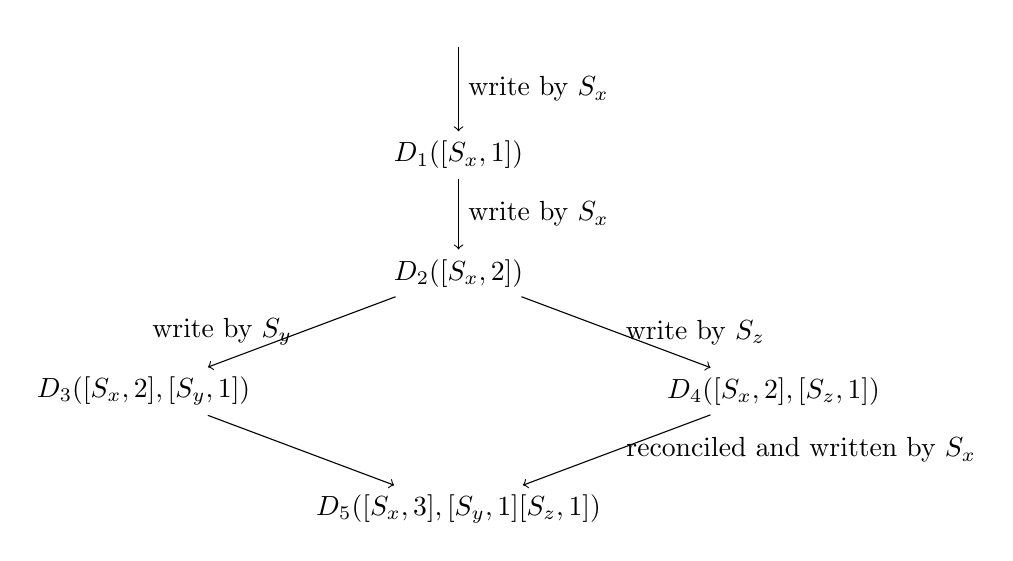
\begin{tikzpicture}[x=2cm, y=1.5cm]
                        \node (o) at (0, 0) {};
                        \node (d1) at (0, -1) {$D_1([S_x, 1])$};
                        \node (d2) at (0, -2) {$D_2([S_x, 2])$};
                        \node (d3) at (-2, -3) {$D_3([S_x, 2], [S_y, 1])$};
                        \node (d4) at (2, -3) {$D_4([S_x, 2], [S_z, 1])$};
                        \node (d5) at (0, -4) {$D_5([S_x, 3], [S_y, 1] [S_z, 1])$};
                        \draw
                        (o) edge[->, right] node{write by $S_x$} (d1)
                        (d1) edge[->, right] node{write by $S_x$} (d2)
                        (d2) edge[->, left] node{write by $S_y$} (d3)
                        (d2) edge[->, right] node{write by $S_z$} (d4)
                        (d3) edge[->] (d5)
                        (d4) edge[->, right] node{reconciled and written by $S_x$} (d5);
                    \end{tikzpicture}
                \end{center}
                Note that not all updates may arrive at all replicas.
                Vector timestamps are used for versioning and reasoning about conflicting updates.
                Each update is associated with a timestamp that records the node (replica) that handled the update.
                The timestamp is incremented in each node.
                The vector clock consists of a set of node and counter pairs.
                A conflicting update occurs when an update is handled by two different nodes concurrently, unaware that they are updating the same key (see the fork in the figure).
                Both components contain the history (the update at $S_x$), and also adds their history.
                \medskip

                There is no ordering between vector timestamps, unless all of the components are ordered.
                For example, $D_2$ is strictly more recent than $D_1$ due to the timestamp, but there is no ordering between $D_3$ and $D_4$ (hence a conflict).
                A reconciliation is done by updating the vector timestamp.
                As such, there is now an ordering again; $D_5$ is strictly more recent than both $D_3$ and $D_4$.
                \medskip

                This only works when we always carry the history of the timestamps (hence the ~context~ parameter in the API).
            \subsubsection*{Nodes}
                As all Dynamo nodes are the same, each needs to deal with;
                \begin{itemize}
                    \itemsep0em
                    \item \textbf{request coordination}
                        \smallskip

                        Accept a read / write query and perform hashing to find the coordinator responsible, and forward to the coordinator.
                    \item \textbf{membership and failure detection}
                        \smallskip

                        Gossip protocol to determine membership.
                    \item \textbf{local persistent storage}
                        \smallskip

                        BigTable had a GFS layer to handle storage.
                        Each node has a storage backend, which can be different embedded databases depending on the need.
                \end{itemize}
            \subsubsection*{Failures}
                It distinguishes between temporary and permanent failures.
                For a permanent failure, it needs to introduce a new replica (one node in the ring has failed, data is lost).
                A new node is added to the preference list, and data is replicated to the new node.
                For a temporary failure, hinted handover can be thought of as temporarily adding a different node to the preference list.
                The assumption is that when the node comes back online, it will take the newly written data (to the temporary node).
            \subsubsection*{Merkle Trees}
                When data is replicated across nodes, a common operation is to discover divergence in the data, and only copy over data where the nodes diverge.
                When a node temporarily disconnects, it will miss a number of updates, but some data still remains.
                As such, we would want to avoid copying over all of the data.
                \medskip

                A Merkle tree can be thought of as a tree of hashes; the parents contain the hashes of their children, and leaves contain hashes of individual keys.
                Parts can be checked without comparing the entire tree - for example if two root hashes are equal, then the trees are equal.
                However, if the root hashes are different, then we can look at the next level down and continue traversing the tree.
                The key-value pairs can be thought of as data blocks, which are hashed.
            \subsubsection*{Evaluation}
                One of the big challenges with the Dynamo design is load balancing (assigning the keys around the wrong).
                Load balancing is done in BigTable by assigning SSTables to tablets.
                If one tablet server is overloaded, tablets can be moved to a server with a lower load.
                This is done by the master, which can see the global state.
                In Dynamo, shifts can only be done around the ring, which can affect the entire ring.
                \medskip

                Both Dynamo and BigTable emphasise writes over reads.
        \subsection*{Spanner}
            Spanner was a response to BigTable and Megastore; and came out of limitations of those systems.
            BigTable was difficult to use, and Megastore was a layer on top of BigTable - the main limitations were the inability to have a complex and evolving schema.
            Dynamo's eventual consistency model gives great scalability and performance, but isn't great from the perspective of the developers (applications need to handle conflicts or may not see the most recent copy of the data) - there was a general pushback in industry against weaker consistency.
            Spanner introduces features that were omitted from distributed systems like BigTable and Dynamo, that developers were used to from traditional databases (such as ACID properties).
            Spanner tries to get the best of both worlds.
            \medskip

            Adopting a scale-out model with sharding, each region can end up with thousands of servers.
            Clients then update the replica in the region geographically closest to them; this leads to the state being inconsistent to the data in a different geographic region.
            A snapshot could be considered a consistent view of the data (on a single machine, block all writes on a read).
            However, this becomes more difficult across multiple machines, as snapshots need to be consistent with each other (globally consistent view of the data).
            With sharding and replication, different operations need a different consistent view over different parts of the data.
            \medskip

            Spanner achieves external consistency; the intuitive way how we'd expect transactions to execute if running on a single machine.
            If transaction $T_1$ commits before another transaction $T_2$ starts, then $T_1$'s commit timestamp is smaller than $T_2$'s (equivalent to linearisability).
            This means that any read that sees $T_2$ must also see $T_1$, there is a total ordering on transactions; a very strong guarantee to achieve on a globally distributed system.
            This creates a total order across all transactions.
            \medskip

            External consistency is achieved by using TrueTime, which acknowledges clock uncertainty (but guarantees a bound) with interval-based global time.
            This is difficult to achieve as there is no global time in a distributed system.
            Logical time enforces a total order (separate from physical time), however these timestamps need to be propagated (all nodes in a system need to agree that logical time has advanced, however, this requires communication).
            On the other hand, wall clock time should be agreed without communication; as long as each node has a source of time, they can individually assign timestamps and keep an ordering on transactions.
            \medskip

            However, as soon as we have local clocks, they will not be perfectly synchronised.
            As soon as two timestamps from different clocks are within the error margin of the clocks, an ordering cannot be defined.
            There is an uncertainty bound with each time, with the difference between the earliest and the latest (in that interval) being $2 \varepsilon$ - timestamps are not points with perfect accuracy, but rather intervals.
            If the uncertainty interval of two timestamps don't overlap, then they are ordered (as good as global time).
            \medskip

            However, Spanner needs to ensure that it never commits two transactions which have overlapping timestamp intervals; this means that the two transactions are not ordered.
            The idea of commit wait is that it needs to wait for whatever the uncertainty bound is.
            \begin{center}
                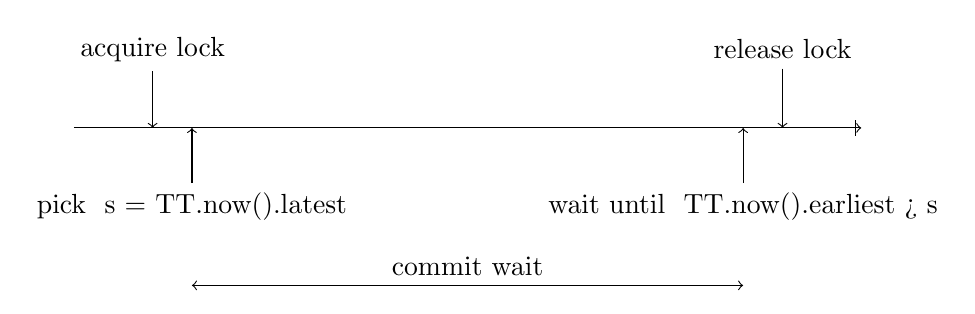
\begin{tikzpicture}
                    \draw (0, 0) edge[-|>] (10, 0);

                    \node (a) at (1, 1) {acquire lock};
                    \node (r) at (9, 1) {release lock};
                    \node (p) at (1.5, -1) {pick ~s = TT.now().latest~};
                    \node (w) at (8.5, -1) {wait until ~TT.now().earliest > s~};
                    \draw
                    (a) edge[->] (1, 0)
                    (r) edge[->] (9, 0)
                    (p) edge[->] (1.5, 0)
                    (w) edge[->] (8.5, 0)
                    (1.5, -2) edge[<->, above] node{commit wait} (8.5, -2);
                \end{tikzpicture}
            \end{center}
            If it waits for the duration of the uncertainty interval and no other node can acquire a lock (so no other node can pick a conflicting timestamp), every node can agree that the two timestamps are ordered.
            This comes with the cost that writes cannot be immediate.
            This works well if the uncertainty is small, as such the performance of the system depends on the accuracy of the times.
            \medskip

            The uncertainty bound needs to be the worst case bound in the system (the most inaccurate clock in the deployment).
            Communication doesn't disappear, but rather is pushed into TrueTime.
            TrueTime is a clock synchronisation protocol that also propagates uncertainty bounds (so that they are globally agreed).
            This is consistent with Lamport's idea that there is no idealised concept of global time.
            \medskip

            Synchronisation is done across a hierarchy (time masters, which are more accurate, with an atomic clock can be used as a source).
            If TrueTime's value of $\varepsilon$ is incorrect, then the ordering is lost, hence inconsistencies can occur and corrupt the data.
            \medskip

            TrueTime can be susceptible to attacks, for example if latency spikes are introduced between data centres, the value of $\varepsilon$ will increase, lowering the throughput.
            Significant engineering went into making the system robust; if TrueTime is disrupted, the performance drops.
            If a network partition occurs in spanner, the uncertainty will begin to increase, leading to the throughput dropping.
            \medskip

            TrueTime gives a very simple API, which gives the following;
            \begin{itemize}
                \itemsep0em
                \item ~now()~ \hfill returns current system time, but also $\varepsilon$ which tells maximum uncertainty
                \item ~after(t)~ \hfill ~true~ if ~t~ is definitely passed
                \item ~before(t)~ \hfill ~true~ if ~d~ definitely not arrived
            \end{itemize}
\end{document}